% Chapter 11

\chapter{Final charged hadrons multiplicities} % Chapter title

\label{ch:mult} % For referencing the chapter elsewhere, use \autoref{ch:name}

%----------------------------------------------------------------------------------------

This chapter is divided in two parts : one is focused on the discussion on the systematic errors, the other presents the final multiplicities of unidentified charged hadrons, charged pions, charged kaons and proton/antiproton extracted from SIDIS of 160 GeV muons off a pure proton target ($lH_2$). These results are obtained from the raw multiplicities of Chapter. \ref{ch:raw} and the correction factors of Chapter. \ref{ch:CF}.

\section{Errors on the RICH unfolding}

The RICH matrices are built using the statistical errors associated to the original probability matrix.

\begin{equation}
M^{\pm}_{RICH}
=
\begin{bmatrix}
\epsilon(\pi \rightarrow \pi)\pm\sigma_{\epsilon(\pi \rightarrow \pi)} & \epsilon(K \rightarrow \pi)\pm\sigma_{\epsilon(K \rightarrow \pi)} & \epsilon(p \rightarrow \pi)\pm\sigma_{\epsilon(p \rightarrow \pi)}\\
\epsilon(\pi \rightarrow K)\pm\sigma_{\epsilon(\pi \rightarrow K)} & \epsilon(K \rightarrow K)\pm\sigma_{\epsilon(K \rightarrow K)} & \epsilon(p \rightarrow K)\pm\sigma_{\epsilon(p \rightarrow K)} \\
\epsilon(\pi \rightarrow p)\pm\sigma_{\epsilon(\pi \rightarrow p)} & \epsilon(K \rightarrow p)\pm\sigma_{\epsilon(K \rightarrow p)} & \epsilon(p \rightarrow p)\pm\sigma_{\epsilon(p \rightarrow p)}
\end{bmatrix}
\end{equation}

As an inversion of the probabilities matrices is done in the analysis, the propagation of errors through the
inversion operation has to be performed. A calculation of the uncertainties on the probabilities yields \cite{} :

\begin{equation}
  [\sigma^{-1}_i]^2 = \epsilon^{-1}_{ip}\epsilon^{-1}_{ir}cov(\epsilon_{pq},\epsilon_{rs})\epsilon^{-1}_{qi}\epsilon^{-1}_{si} + [\epsilon^{-1}_{ik}\sigma_k]^2
\end{equation}

This equation leads to the inverse error matrices with associated statistical errors :

\begin{equation}
[M^{\pm}_{RICH}]^{-1}
=
\begin{bmatrix}
\epsilon^{-1}(\pi \rightarrow \pi)\pm\sigma^{-1}_{\epsilon(\pi \rightarrow \pi)} & \epsilon^{-1}(K \rightarrow \pi)\pm\sigma^{-1}_{\epsilon(K \rightarrow \pi)} & \epsilon^{-1}(p \rightarrow \pi)\pm\sigma^{-1}_{\epsilon(p \rightarrow \pi)}\\
\epsilon^{-1}(\pi \rightarrow K)\pm\sigma^{-1}_{\epsilon(\pi \rightarrow K)} & \epsilon^{-1}(K \rightarrow K)\pm\sigma^{-1}_{\epsilon(K \rightarrow K)} & \epsilon^{-1}(p \rightarrow K)\pm\sigma^{-1}_{\epsilon(p \rightarrow K)} \\
\epsilon^{-1}(\pi \rightarrow p)\pm\sigma^{-1}_{\epsilon(\pi \rightarrow p)} & \epsilon^{-1}(K \rightarrow p)\pm\sigma^{-1}_{\epsilon(K \rightarrow p)} & \epsilon^{-1}(p \rightarrow p)\pm\sigma^{-1}_{\epsilon(p \rightarrow p)}
\end{bmatrix}
\end{equation}

%----------------------------------------------------------------------------------------

\section{Summary of systematic studies}

The various systematic studies that were performed are summarized hereafter.

%------------------------------------------------

\subsection{Error associated to the stability of data over time}

The data samples used in the analysis were recorded over a period of 5 weeks. As a quality check, the sum and ratio of multiplicities in the different weeks were compared to the sum and ratio of multiplicities over the overall 5 weeks of data and the multiplicities averaged over y were compared period by period. The compatibility between weeks was found to be below the 1\% level within statistical fluctuations. Consequently, no systematic error will be assigned for the data compatibility.

%------------------------------------------------

\subsection{Error associated to the stability of data over beam charge}

The data samples used in the analysis were recorded with two different beam charge. As a quality check, the multiplicities averaged over y were compared for both beam charge. The compatibility between the two beam charge was found to be below the 1\% level within statistical fluctuations. Consequently, no systematic error will be assigned for the beam charge change.

%------------------------------------------------

\subsection{Error associated to Monte Carlo sample : DJANGOH dependence}

To determine the acceptance dependence with the physical model chosen, different PDF sets were used to generate different MC samples. Moreover different JETSET parameters were also used \cite{}. For each sample the acceptance is calculated and the hadron multiplicities are the corrected with each acceptance. The systematic uncertainty on the acceptance, considering two acceptances $A^h$ and $A'^h$, is estimed in each kinematic bin ($x$,$y$,$z$) :

\begin{equation}
  \sigma^{A^h}_{syst} \leq \frac{\frac{A'^h}{A^h}-1}{2}M^h_{corr_acc}
\end{equation}

The value of $\sigma^{A^h}_{syst}$ was found to be of $\sim$ 5\%.

Another error concerns the z-vertex dependence : the target can be separated into 4 different parts and the sum of multiplicities extracted from each part is then compared (Fig. \ref{pic:Zvertexsum} and \ref{pic:Zvertexratio}). From this comparison, a conservative systematic error of $\sim$ 5\% was derived.

In the end, a total systematic uncertainty of $\sim$ 10\% is put on the acceptance.

%------------------------------------------------

\subsection{Error associated to the diffractive vector meson correction}

In HEPGEN, the cross section for exclusive vector meson production is normalized to the GPD model of Goloskokov and Kroll. The theoretical uncertainty on the predicted cross section close to COMPASS kinematics is around 30\% \cite{Goloskokov}. Propagating this uncertainty leads to a maximum relative uncertainty under 6\%.
The method for the correction of nuclear effects maily changes the shape of the $p_T^2$ distribution with respect to the diffractive vector meson production on a free nucleon. It assumes that the $p_T^2$-integrated nuclear cross-section per nucleon for exclusive events is the same as the $p_T^2$-integrated nuclear cross section for a free nucleon. According to A. Sandacz \cite{Hepgen}, the systematic uncertainty due to this assumption is a few percent.

%----------------------------------------------------------------------------------------

\section{Charged hadrons multiplicities ($h^{\pm}$,$\pi^{\pm}$,$K^{\pm}$,$p/\bar{p}$)}

The multiplicities presented in the following sections are with all the correction presented before viz. :

\begin{equation}
  	M^h_{Final}(x,y,z) = M^h_{raw}(x,y,z)\frac{\eta^h(x,y,z)}{A^h(x,y,z)}B^h(x,y,z)
\end{equation}

The $x$,$y$ and $z$ binning is given in Table. \ref{tab:binning}. $A^h$ corresponds to the acceptance correction (Section. \ref{sec:Acc}), $\eta^h$ to the radiative correction factor (Section. \ref{sec:rcf}) and $B^h$ to the diffractive vector meson correction factor (Section. \ref{sec:DVMf}). The statistical error propagation is performed assuming that all corrections are independent :

\begin{equation}
\begin{split}
		E^2_{Final} = \bigg( \frac{RC.VM}{Acc} \bigg)^2 E^2_{Raw} + \bigg(\frac{RC.VM.Raw}{Acc^2} \bigg)^2 E^2_{Acc} \\
		+ \bigg(\frac{RC.Raw}{Acc} \bigg)^2 E^2_{VM} + \bigg(\frac{VM.Raw}{Acc} \bigg)^2 E^2_{RC}
\end{split}
\end{equation}

The corresponding systematic error from the different sources are added quadratically. The largest contribution in most bins comes from the systematic uncertainty on the acceptance.

\subsection{Unidentified charged hadron multiplicities}

The unidentified charged hadron multiplicities $M^{h^{\pm}}$ are shown in Fig. \ref{pic:mhp} and \ref{pic:mhm} in function of $z$, in bins of $x$ and staggered vertically with $y$. A strong $z$ dependence is observed for all ($x$,$y$) bins as well as a small dependence with $x$. The $Q^2$ values are in the range 1 to 30 (GeV/$c$)$^2$. $M^{h^+}$ and $M^{h^-}$ have 300 data points each. The statistical uncertainties are too small to be visible in almost all kinematic bins. The bands at the bottom of each $x$ bin panel are the systematic errors for the bin 0.3$< y <$0.5 (bin that covers the largest $z$ range).

\begin{figure}[!h]
	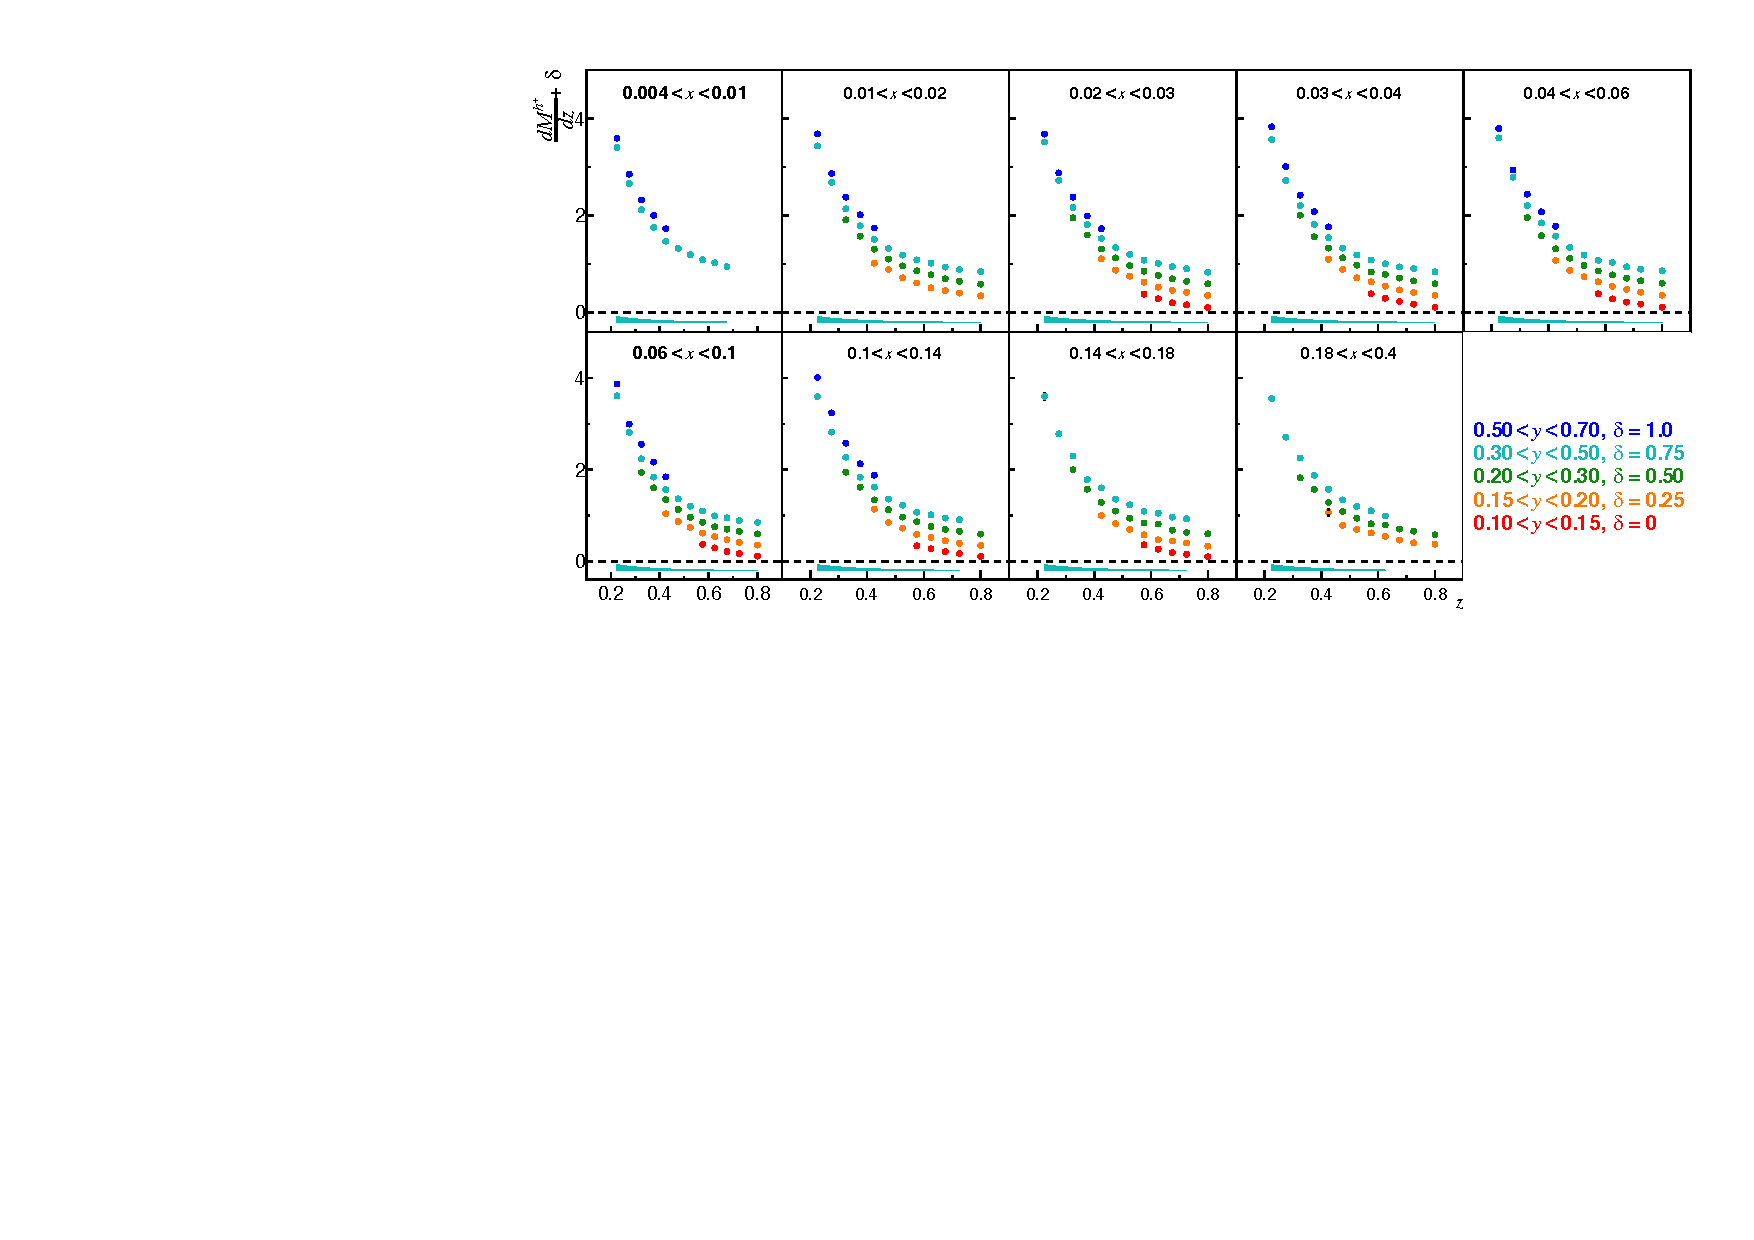
\includegraphics[scale=0.85]{./gfx/hp.pdf}
	\caption{Unidentified positive hadron multiplicities (with all corrections) as a function of $z$ in bins of $x$ staggered vertically with $y$.}
	\label{pic:mhp}
\end{figure}

\begin{figure}[!h]
	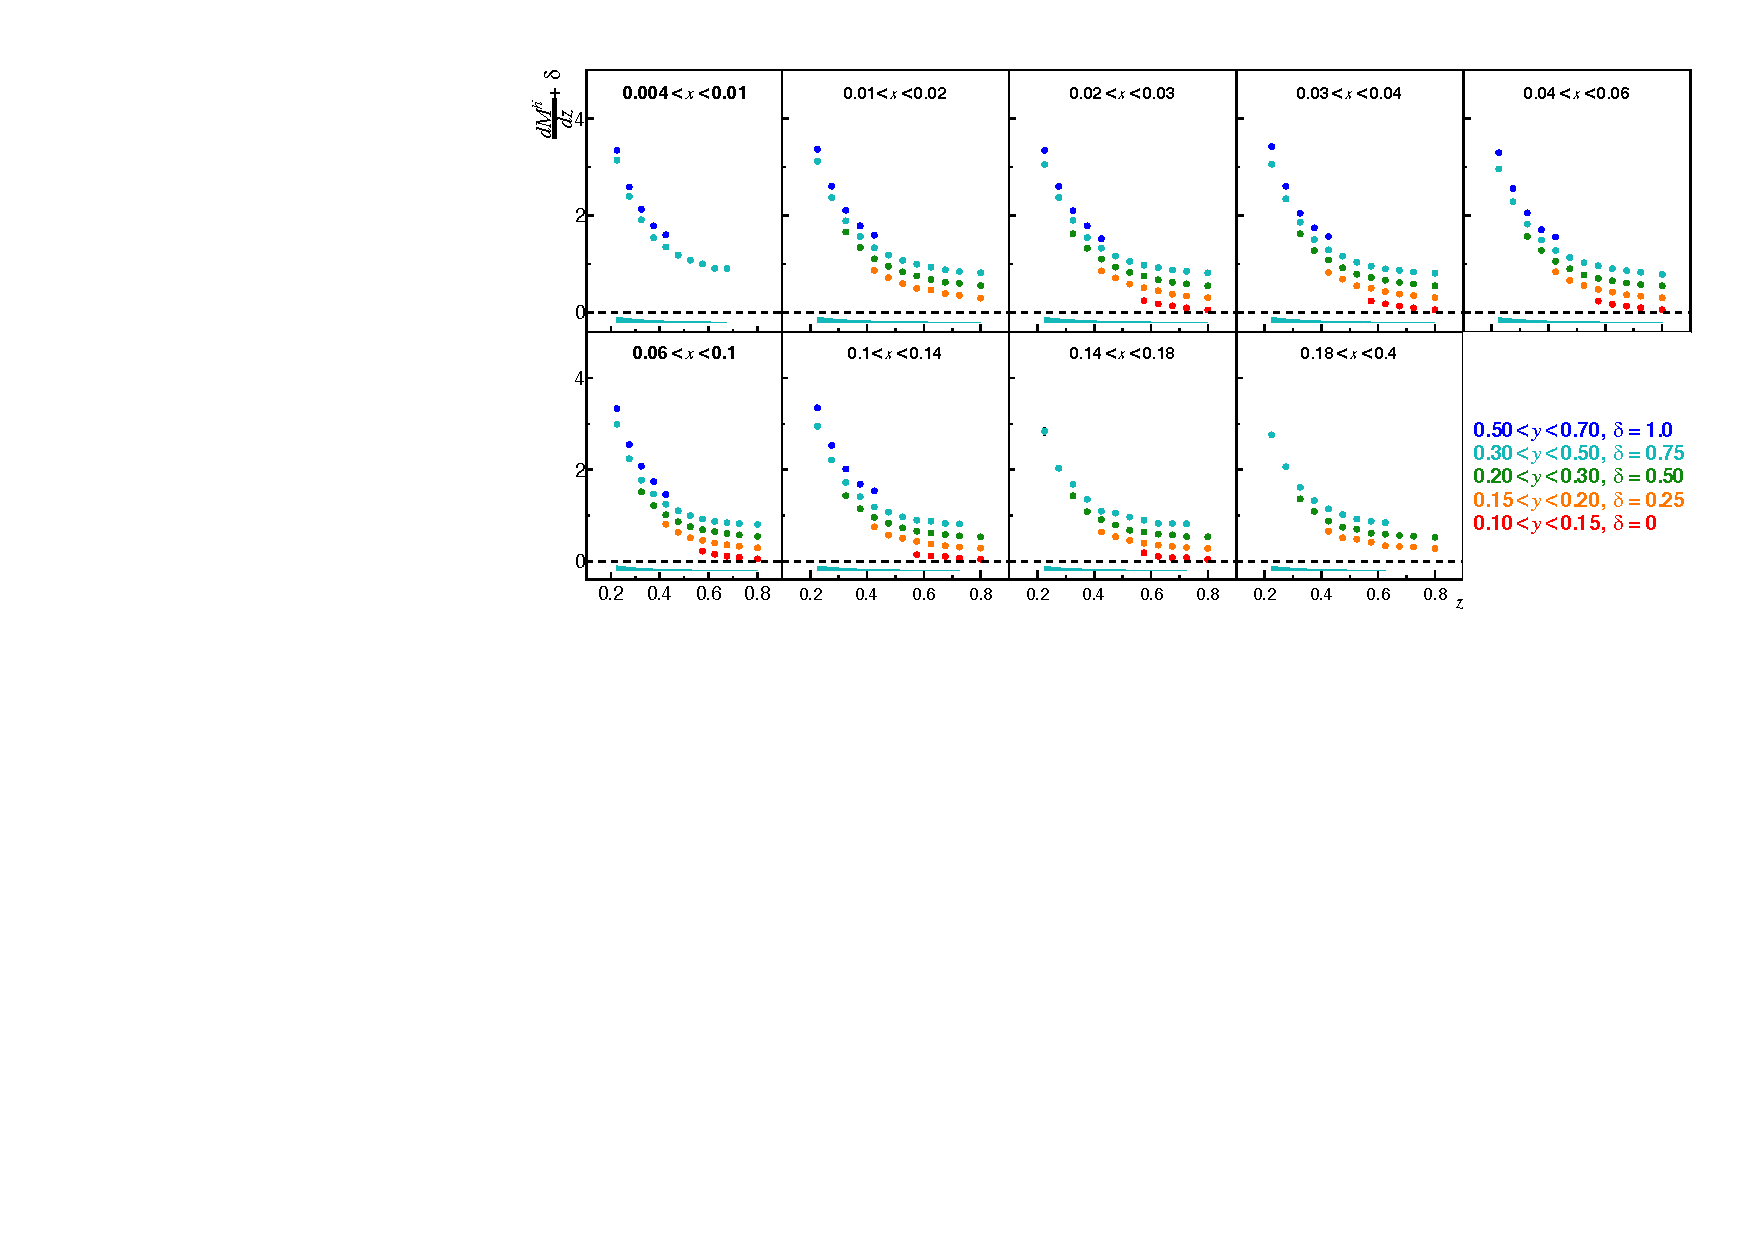
\includegraphics[scale=0.85]{./gfx/hm.pdf}
	\caption{Unidentified positive hadron multiplicities (with all corrections) as a function of $z$ in bins of $x$ staggered vertically with $y$.}
	\label{pic:mhm}
\end{figure}

When removing the $y$ staggering on the previous results, one can see that all data points for different $y$ bins are overlapping (Fig. \ref{pic:mhnoy}). That means that our multiplicities results have no $y$ dependence and can then be averaged over $y$, using the square of the statistical error as weight. Then the multiplicities are displayed as a function of $z$ and in bins of $x$. With Fig. \ref{pic:mhyavg} an asymmetry between $h^+$ and $h^-$ is observed, increasing with $x$.

\begin{figure}[!h]
	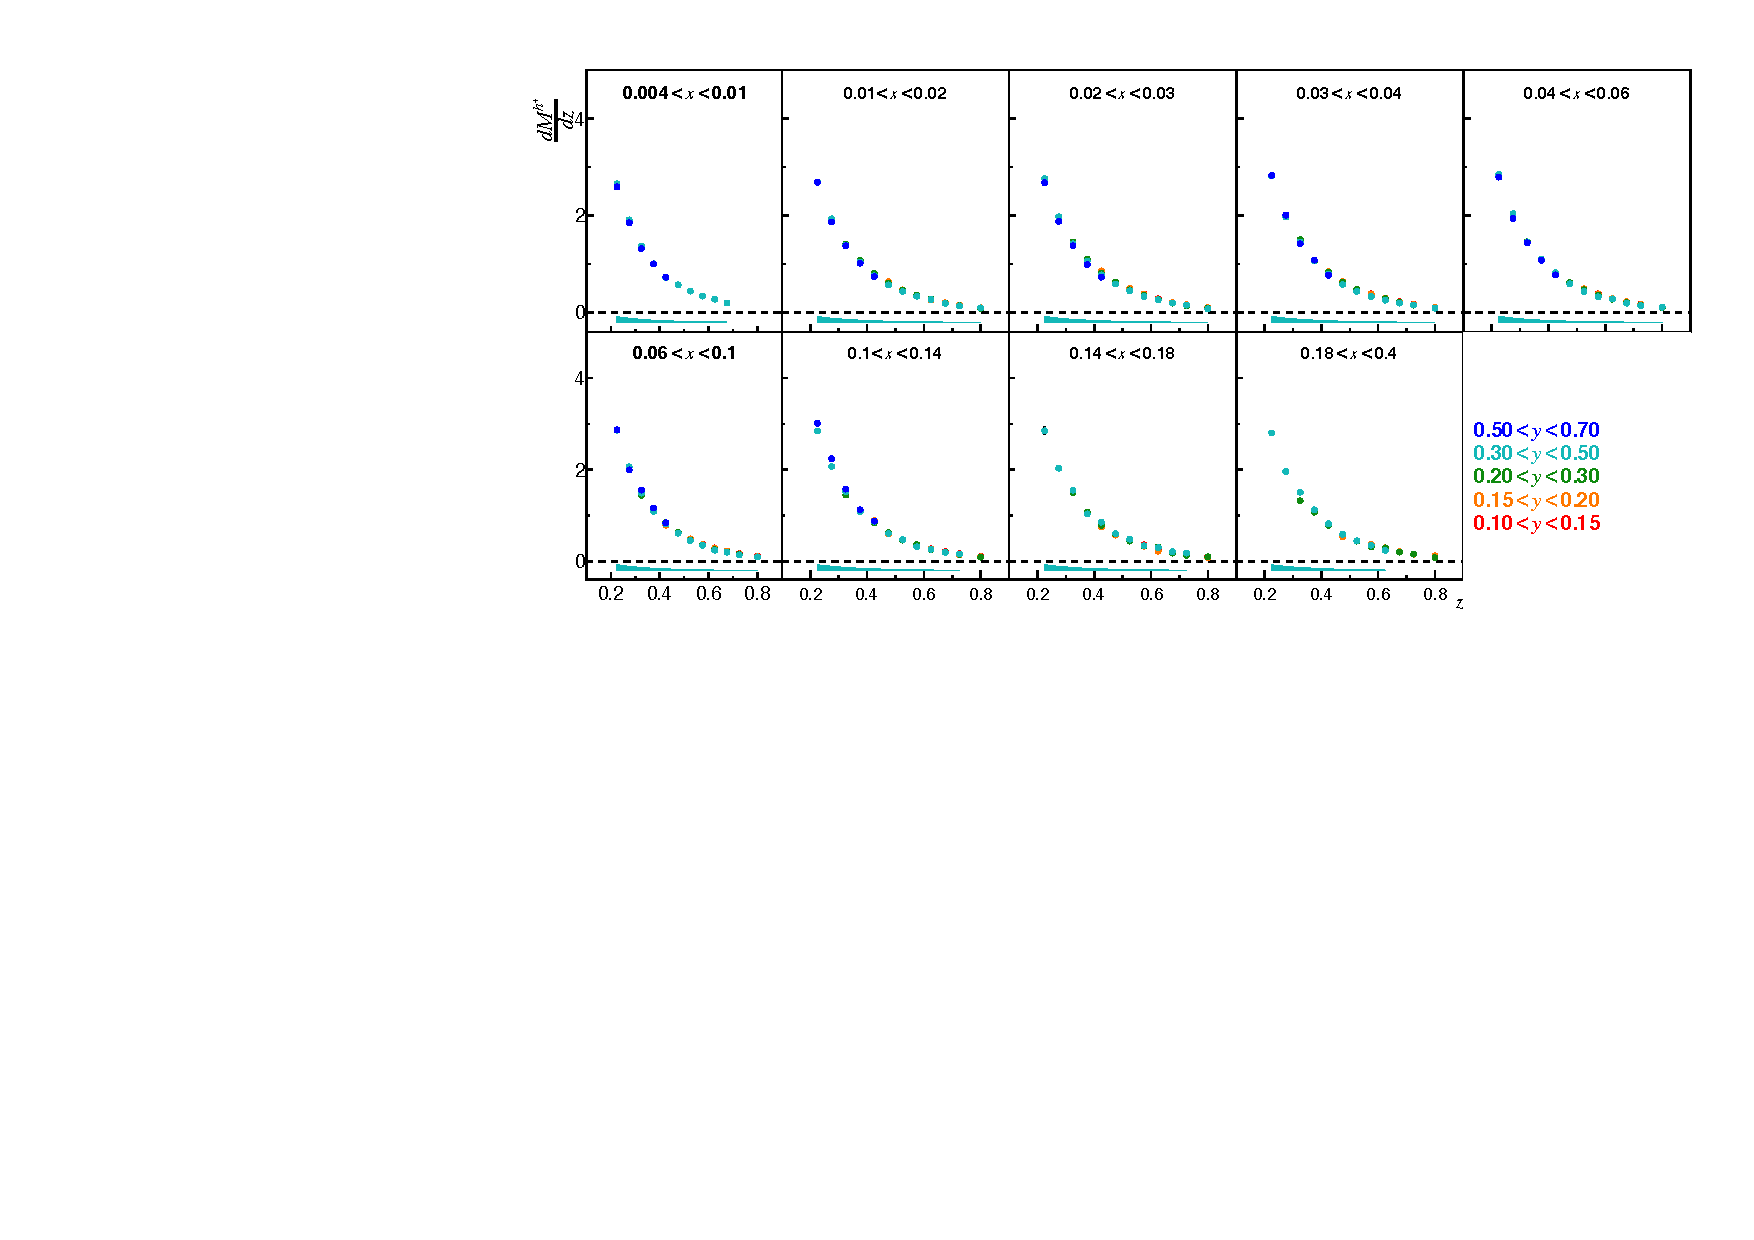
\includegraphics[scale=0.85]{./gfx/hnoystag.pdf}
	\caption{Unidentified positive hadron multiplicities (with all corrections) as a function of $z$ in bins of $x$. The vertical staggering with $y$ has been suppressed showing that different $y$ bins overlap.}
	\label{pic:mhnoy}
\end{figure}

\begin{figure}[!h]
	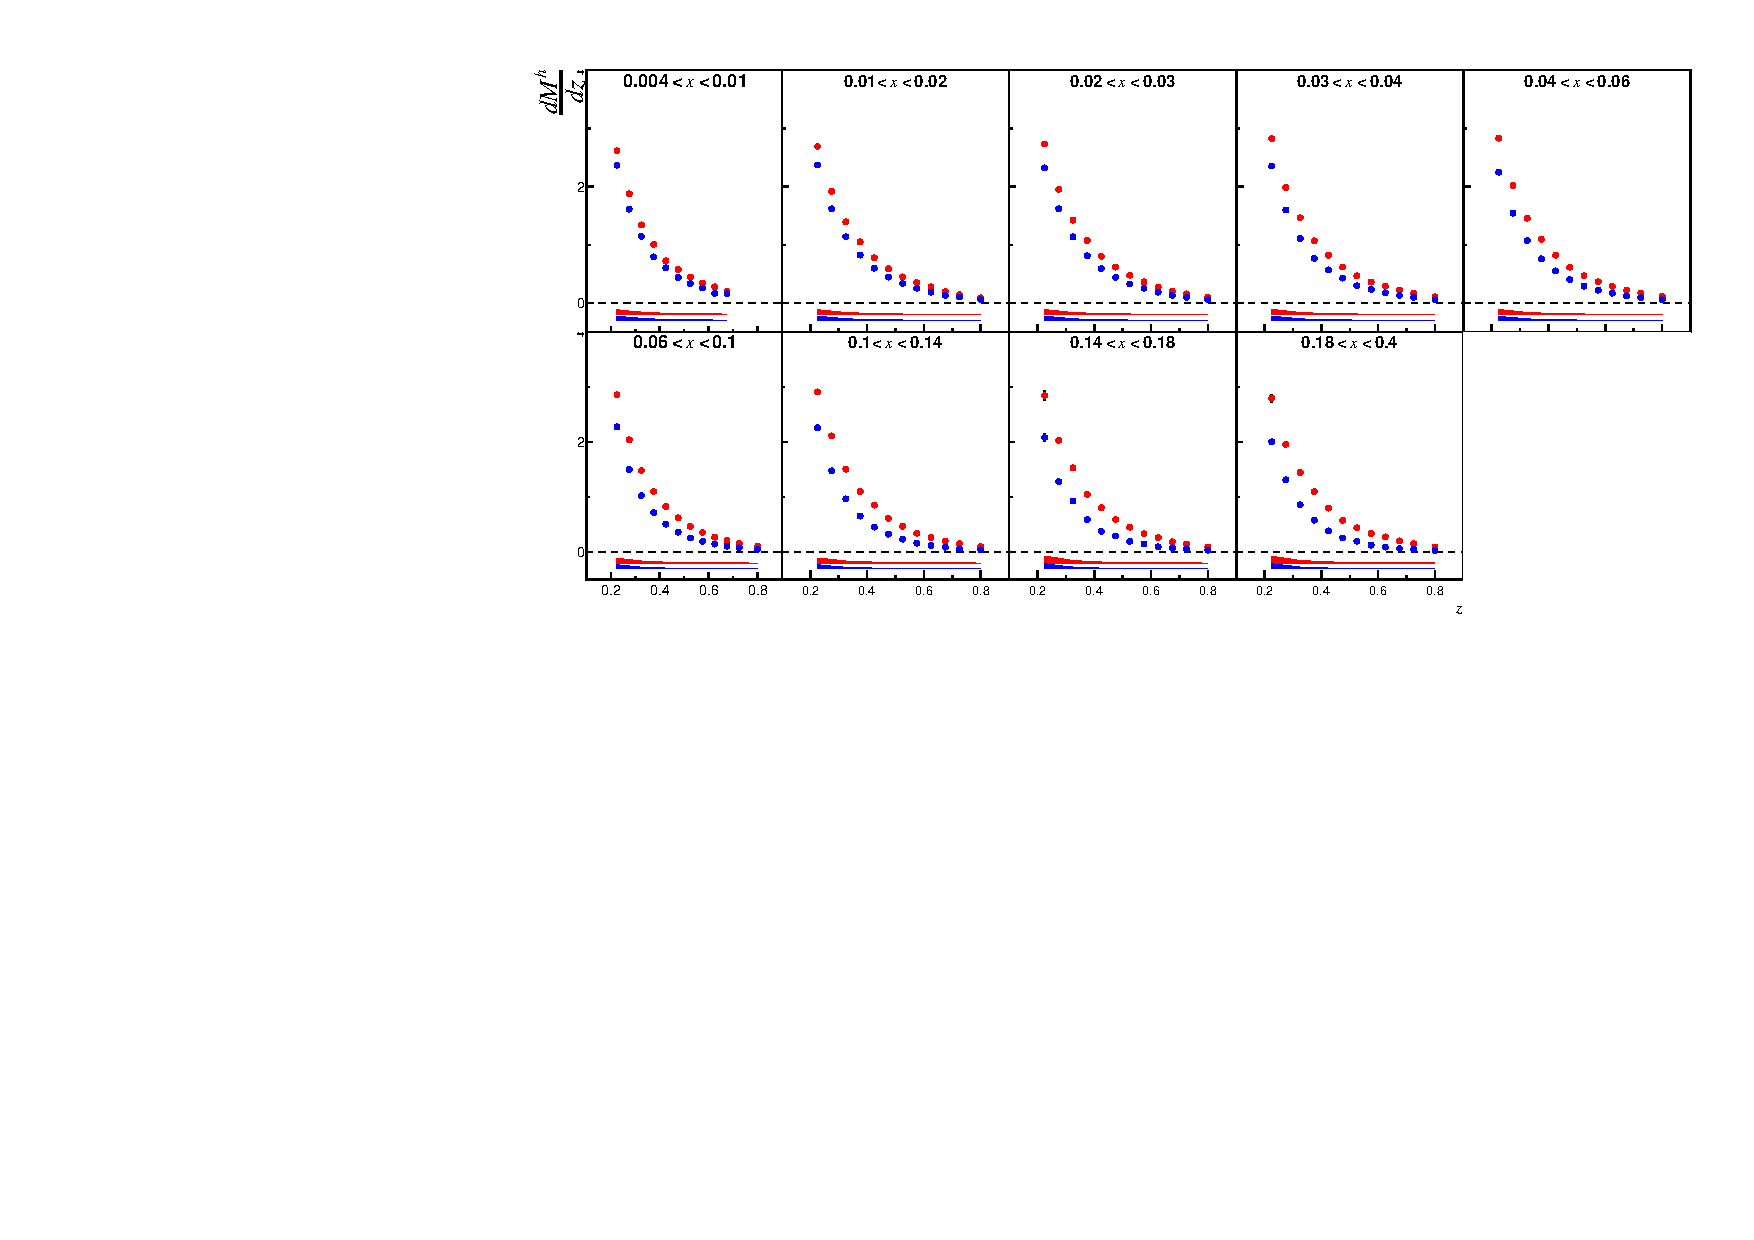
\includegraphics[scale=0.85]{./gfx/hyavg.pdf}
	\caption{Unidentified positive (red) and negative (blue) hadron multiplicities (with all corrections) averaged over $y$ as a function of $z$ in bins of $x$.}
	\label{pic:mhyavg}
\end{figure}

\newpage
\subsection{Charged pion multiplicities}

The charged pion multiplicities $M^{\pi^{\pm}}$ are shown in Fig. \ref{pic:mpip} and \ref{pic:mpim} in function of $z$, in bins of $x$ and staggered vertically with $y$. A strong $z$ dependence is observed for all ($x$,$y$) bins as well as a small dependence with $x$. $M^{\pi^+}$ and $M^{\pi^-}$ have 300 data points each. The statistical uncertainties are too small to be visible in almost all kinematic bins. The bands at the bottom of each $x$ bin panel are the systematic errors for the bin 0.3$< y <$0.5 (bin that covers the largest $z$ range).

\begin{figure}[!h]
	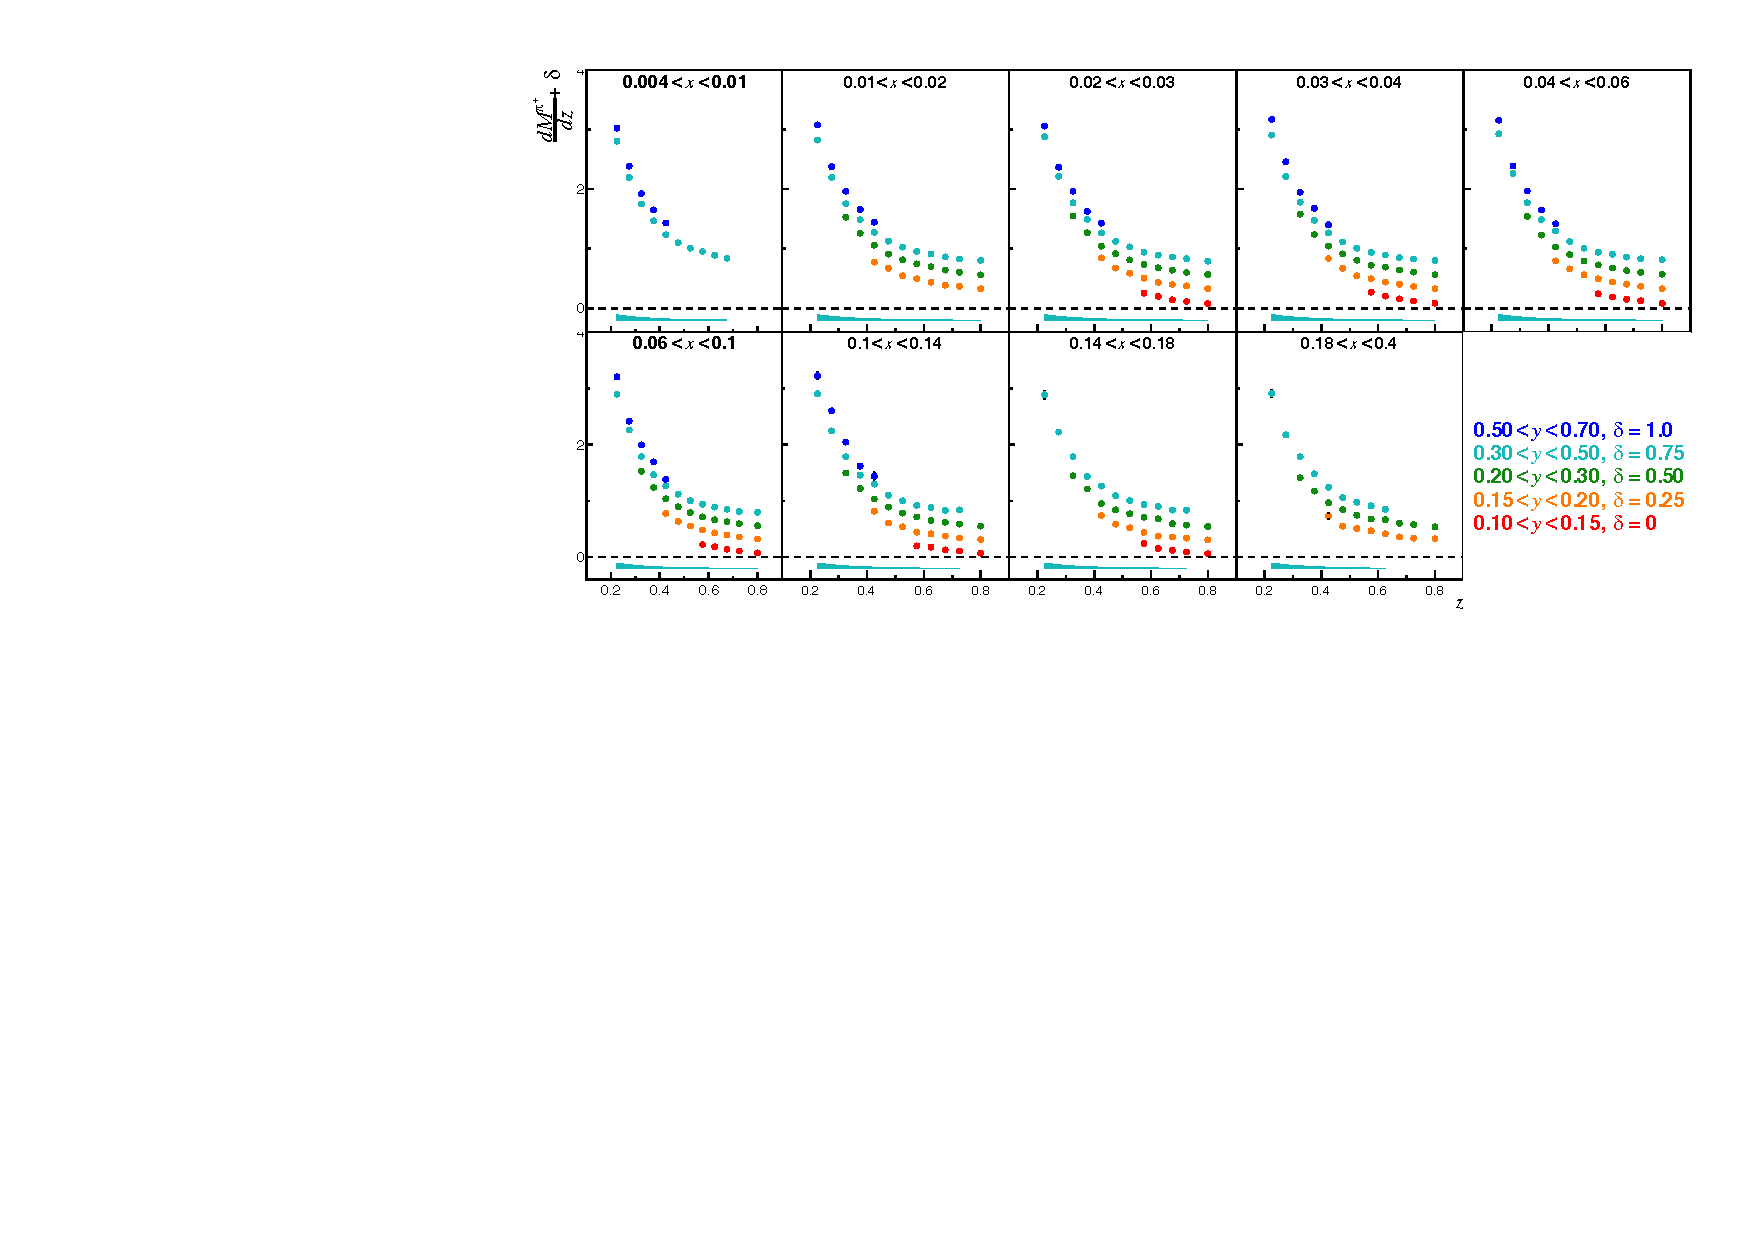
\includegraphics[scale=0.85]{./gfx/pip.pdf}
	\caption{Positive pion multiplicities (with all corrections) as a function of $z$ in bins of $x$ staggered vertically with $y$.}
	\label{pic:mpip}
\end{figure}

\begin{figure}[!h]
	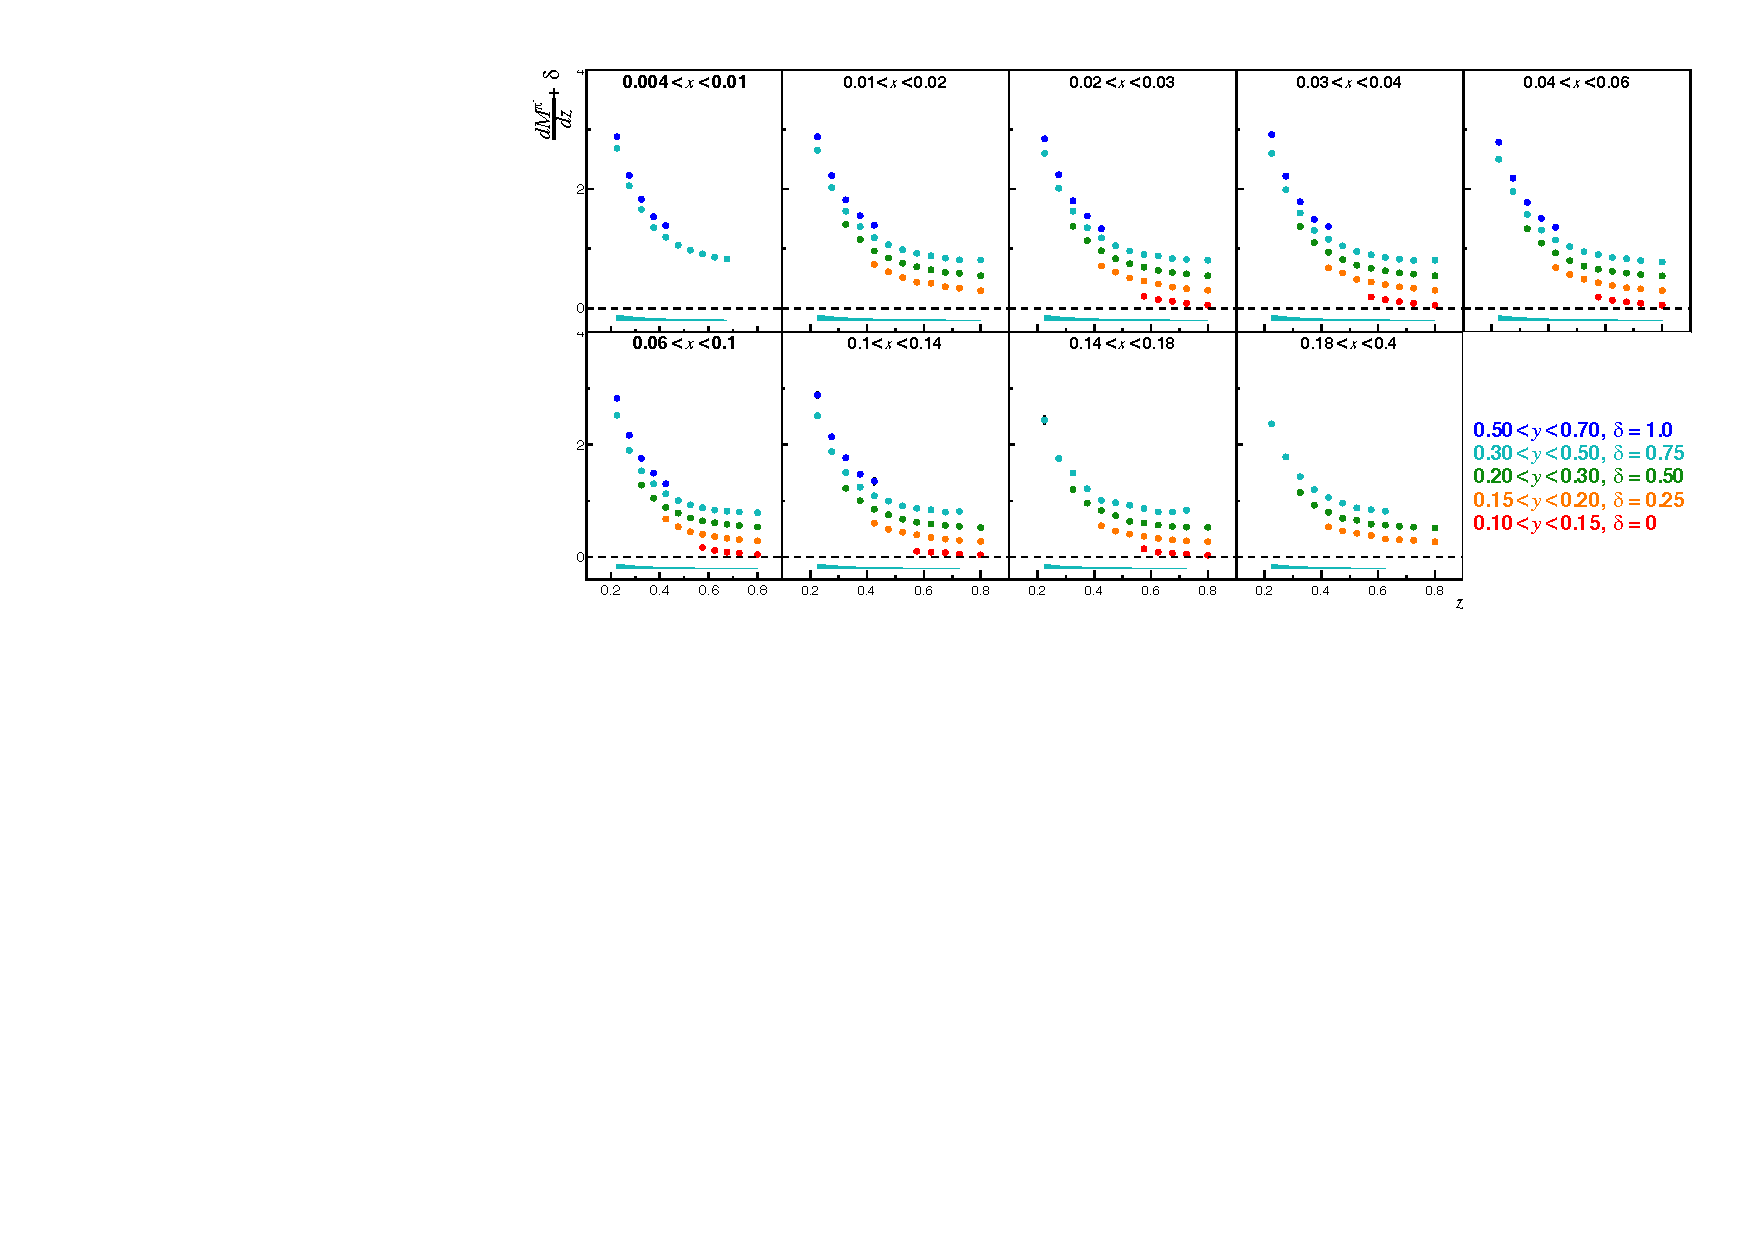
\includegraphics[scale=0.85]{./gfx/pim.pdf}
	\caption{Negative pion multiplicities (with all corrections) as a function of $z$ in bins of $x$ staggered vertically with $y$.}
	\label{pic:mpim}
\end{figure}

The y-averaged multiplicities are displayed as a function of $z$ and in bins of $x$. With Fig. \ref{pic:mpiyavg} an asymmetry between $\pi^+$ and $\pi^-$ is observed, increasing with $x$. Having more $\pi^+$ than $\pi^-$ is due to the fact there is a dominant $u$ quark distribution in the target.

\begin{figure}[!h]
	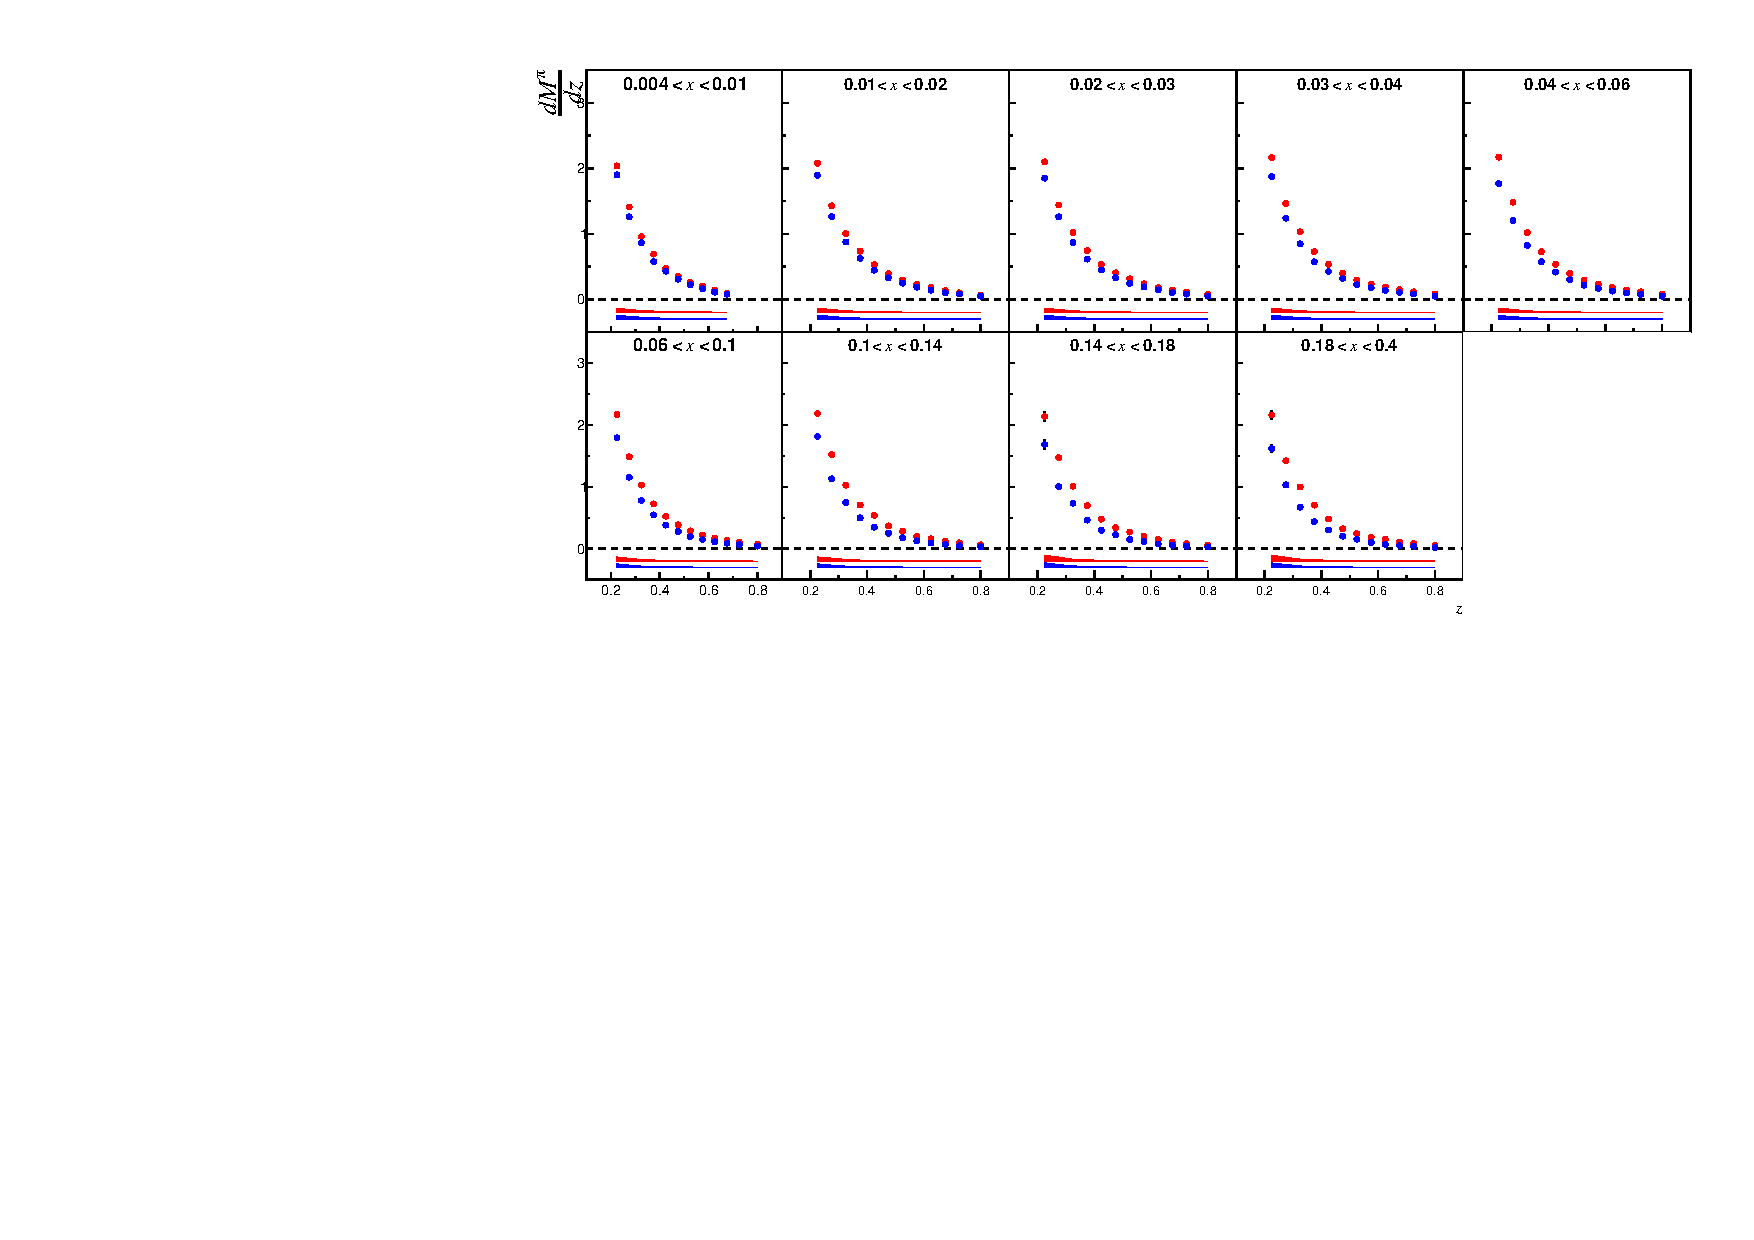
\includegraphics[scale=0.85]{./gfx/piyavg.pdf}
	\caption{Positive (red) and negative (blue) pion multiplicities (with all corrections) averaged over $y$ as a function of $z$ in bins of $x$.}
	\label{pic:mpiyavg}
\end{figure}

\subsection{Charged kaon multiplicities}

The charged kaon multiplicities $M^{K^{\pm}}$ are shown in Fig. \ref{pic:mpip} and \ref{pic:mpim} in function of $z$, in bins of $x$ and staggered vertically with $y$. A strong $z$ dependence is observed for all ($x$,$y$) bins as well as a small dependence with $x$. $M^{K^+}$ and $M^{K^-}$ have 300 data points each. The statistical uncertainties are too small to be visible in almost all kinematic bins. The bands at the bottom of each $x$ bin panel are the systematic errors for the bin 0.3$< y <$0.5 (bin that covers the largest $z$ range).

\begin{figure}[!h]
	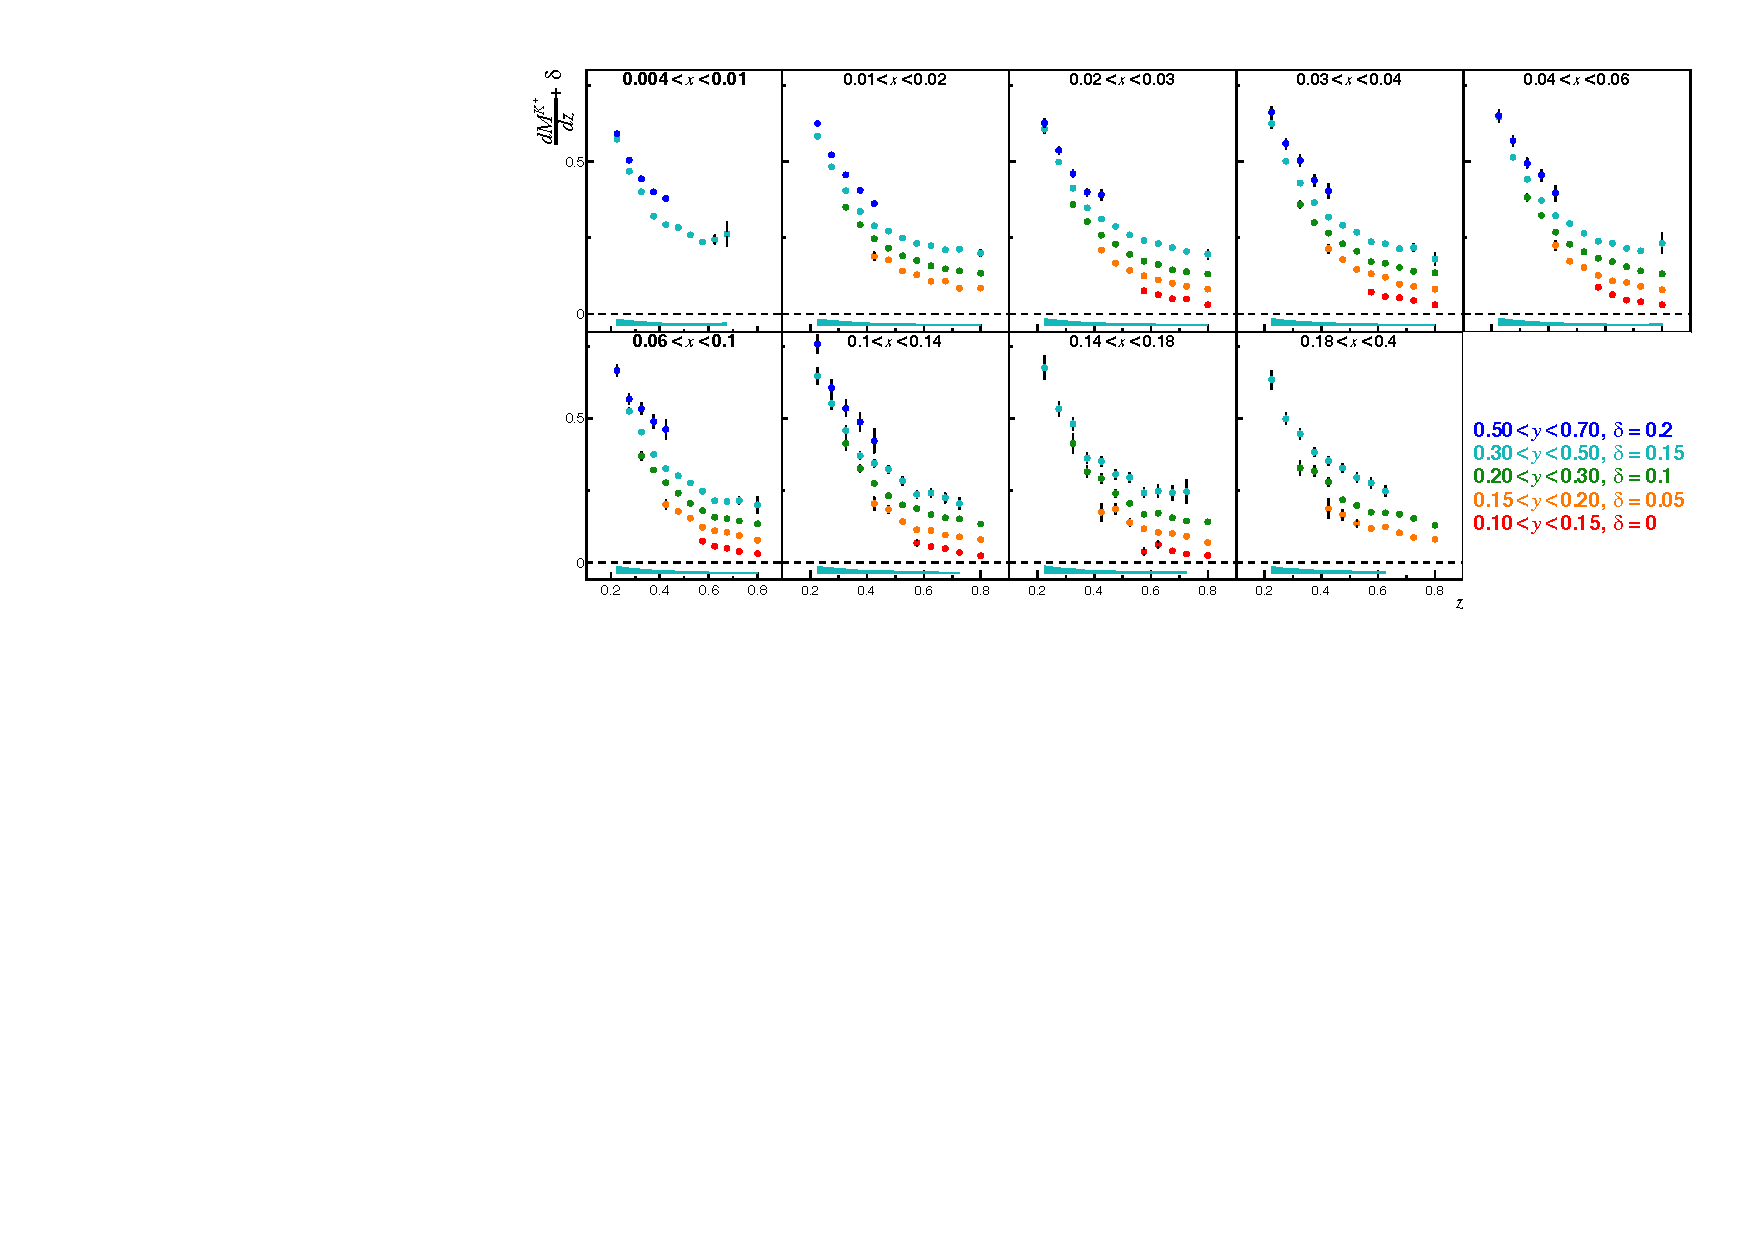
\includegraphics[scale=0.85]{./gfx/Kp.pdf}
	\caption{Positive kaon multiplicities (with all corrections) as a function of $z$ in bins of $x$ staggered vertically with $y$.}
	\label{pic:mkp}
\end{figure}

\begin{figure}[!h]
	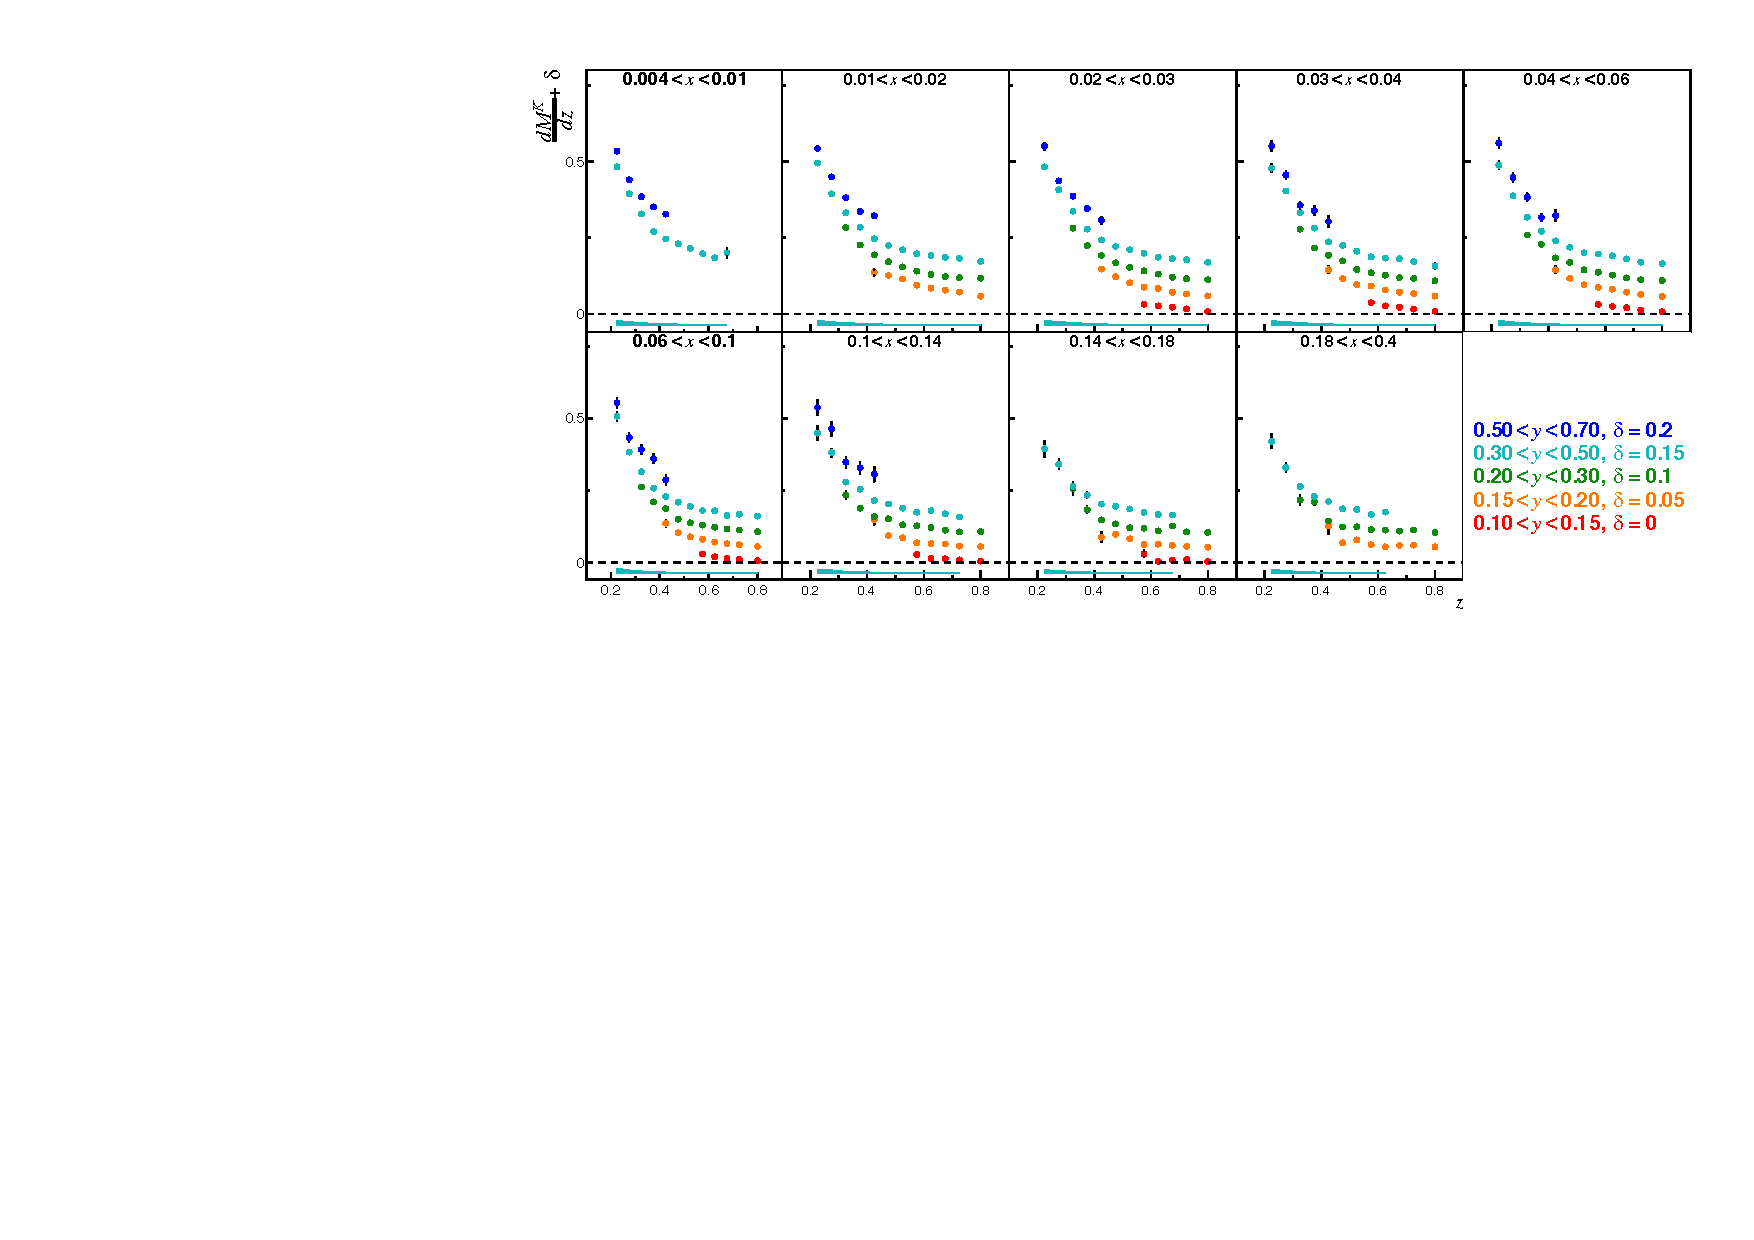
\includegraphics[scale=0.85]{./gfx/Km.pdf}
	\caption{Negative kaon multiplicities (with all corrections) as a function of $z$ in bins of $x$ staggered vertically with $y$.}
	\label{pic:mkm}
\end{figure}

The y-averaged multiplicities are displayed as a function of $z$ and in bins of $x$. With Fig. \ref{pic:mkyavg} an asymmetry between $K^+$ and $K^-$ is observed, increasing with $x$. Having more $K^+$ than $K^-$ is due to the fact there is a dominant $u$ quark distribution in the target.

\begin{figure}[!h]
	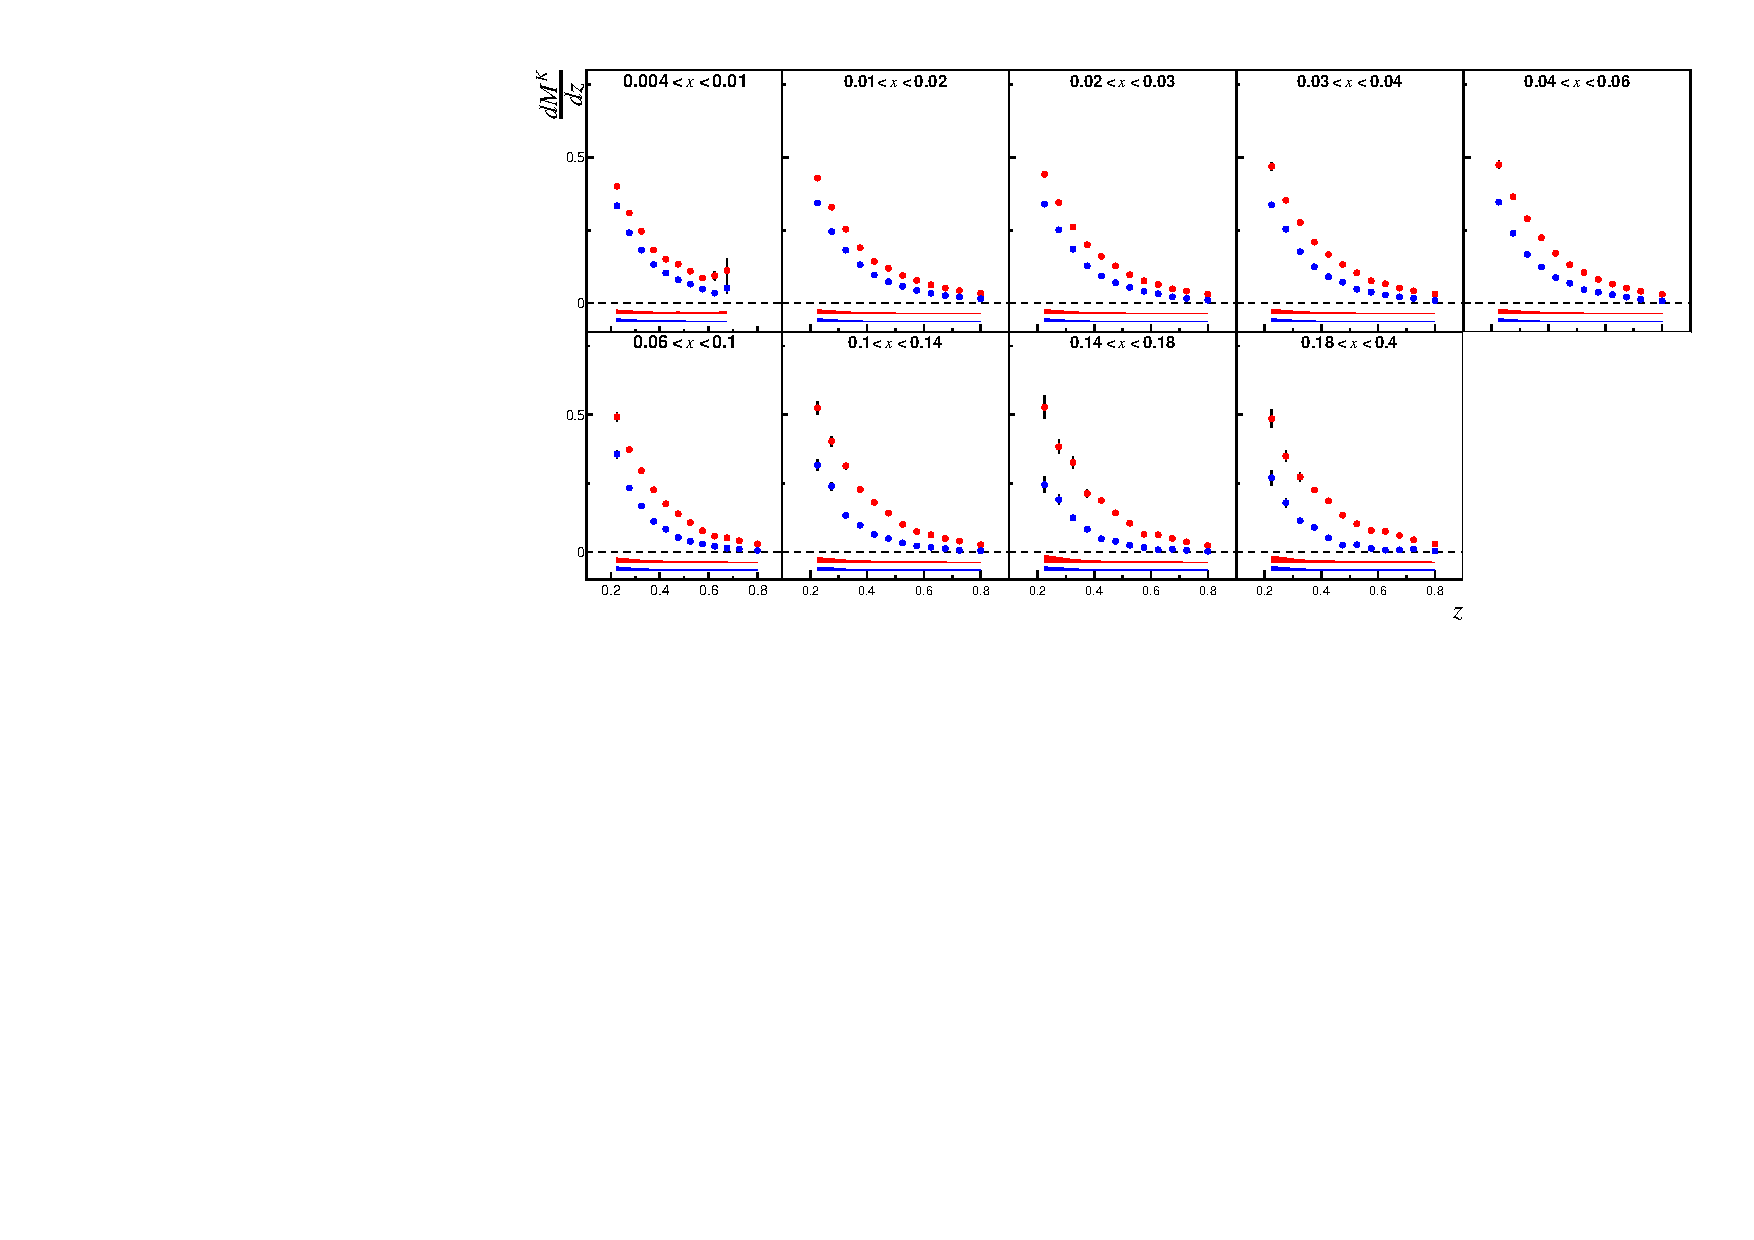
\includegraphics[scale=0.85]{./gfx/Kyavg.pdf}
	\caption{Positive (red) and negative (blue) kaon multiplicities (with all corrections) averaged over $y$ as a function of $z$ in bins of $x$.}
	\label{pic:mkyavg}
\end{figure}

\subsection{Proton/Antiproton multiplicities}

The proton/antiproton multiplicities $M^{p/\bar{p}}$ are shown in Fig. \ref{pic:mpp} and \ref{pic:mpm} in function of $z$, in bins of $x$ and staggered vertically with $y$. A strong $z$ dependence is observed for all ($x$,$y$) bins as well as a small dependence with $x$. $M^{K^+}$ and $M^{K^-}$ have 300 data points each. The statistical uncertainties are too small to be visible in almost all kinematic bins. The bands at the bottom of each $x$ bin panel are the systematic errors for the bin 0.3$< y <$0.5 (bin that covers the largest $z$ range).

\begin{figure}[!h]
	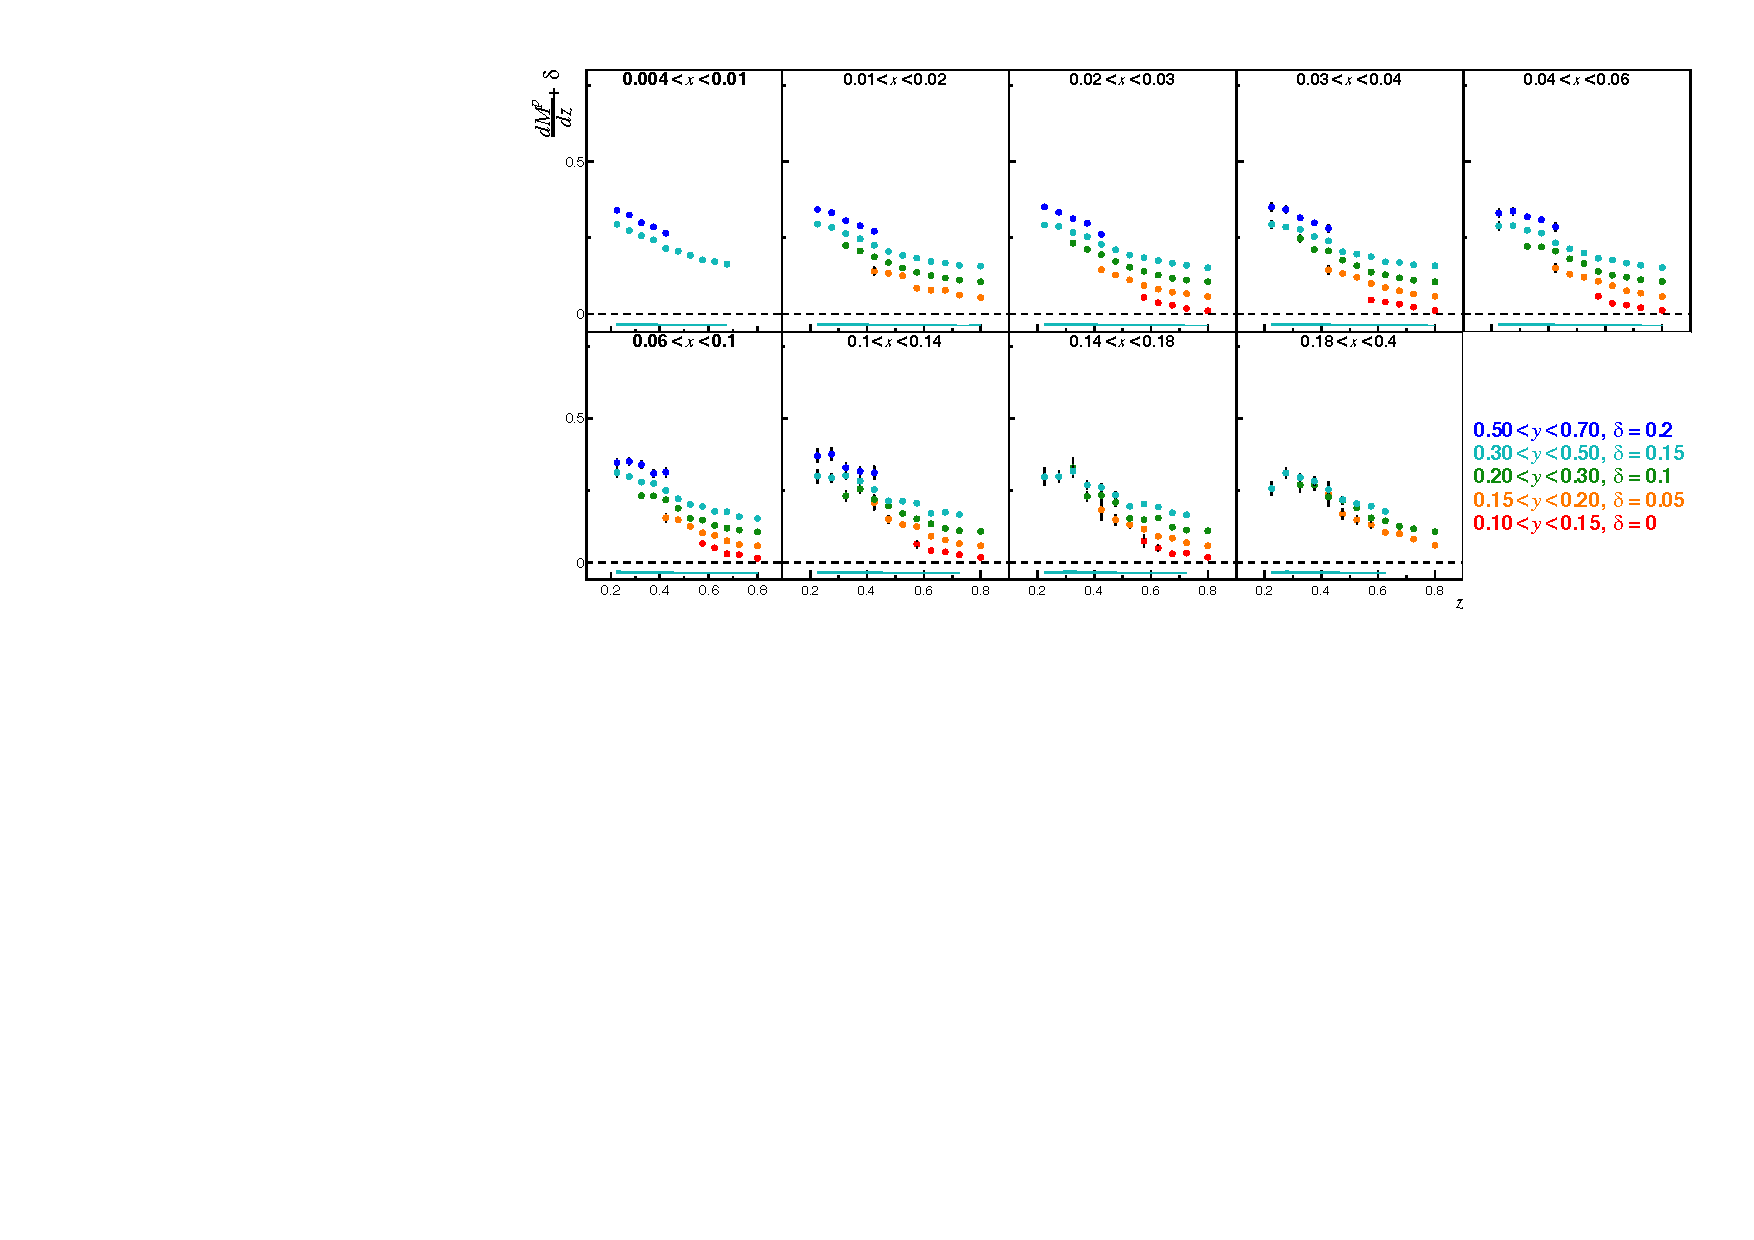
\includegraphics[scale=0.85]{./gfx/pp.pdf}
	\caption{Proton multiplicities (with all corrections) as a function of $z$ in bins of $x$ staggered vertically with $y$.}
	\label{pic:mpp}
\end{figure}

\begin{figure}[!h]
	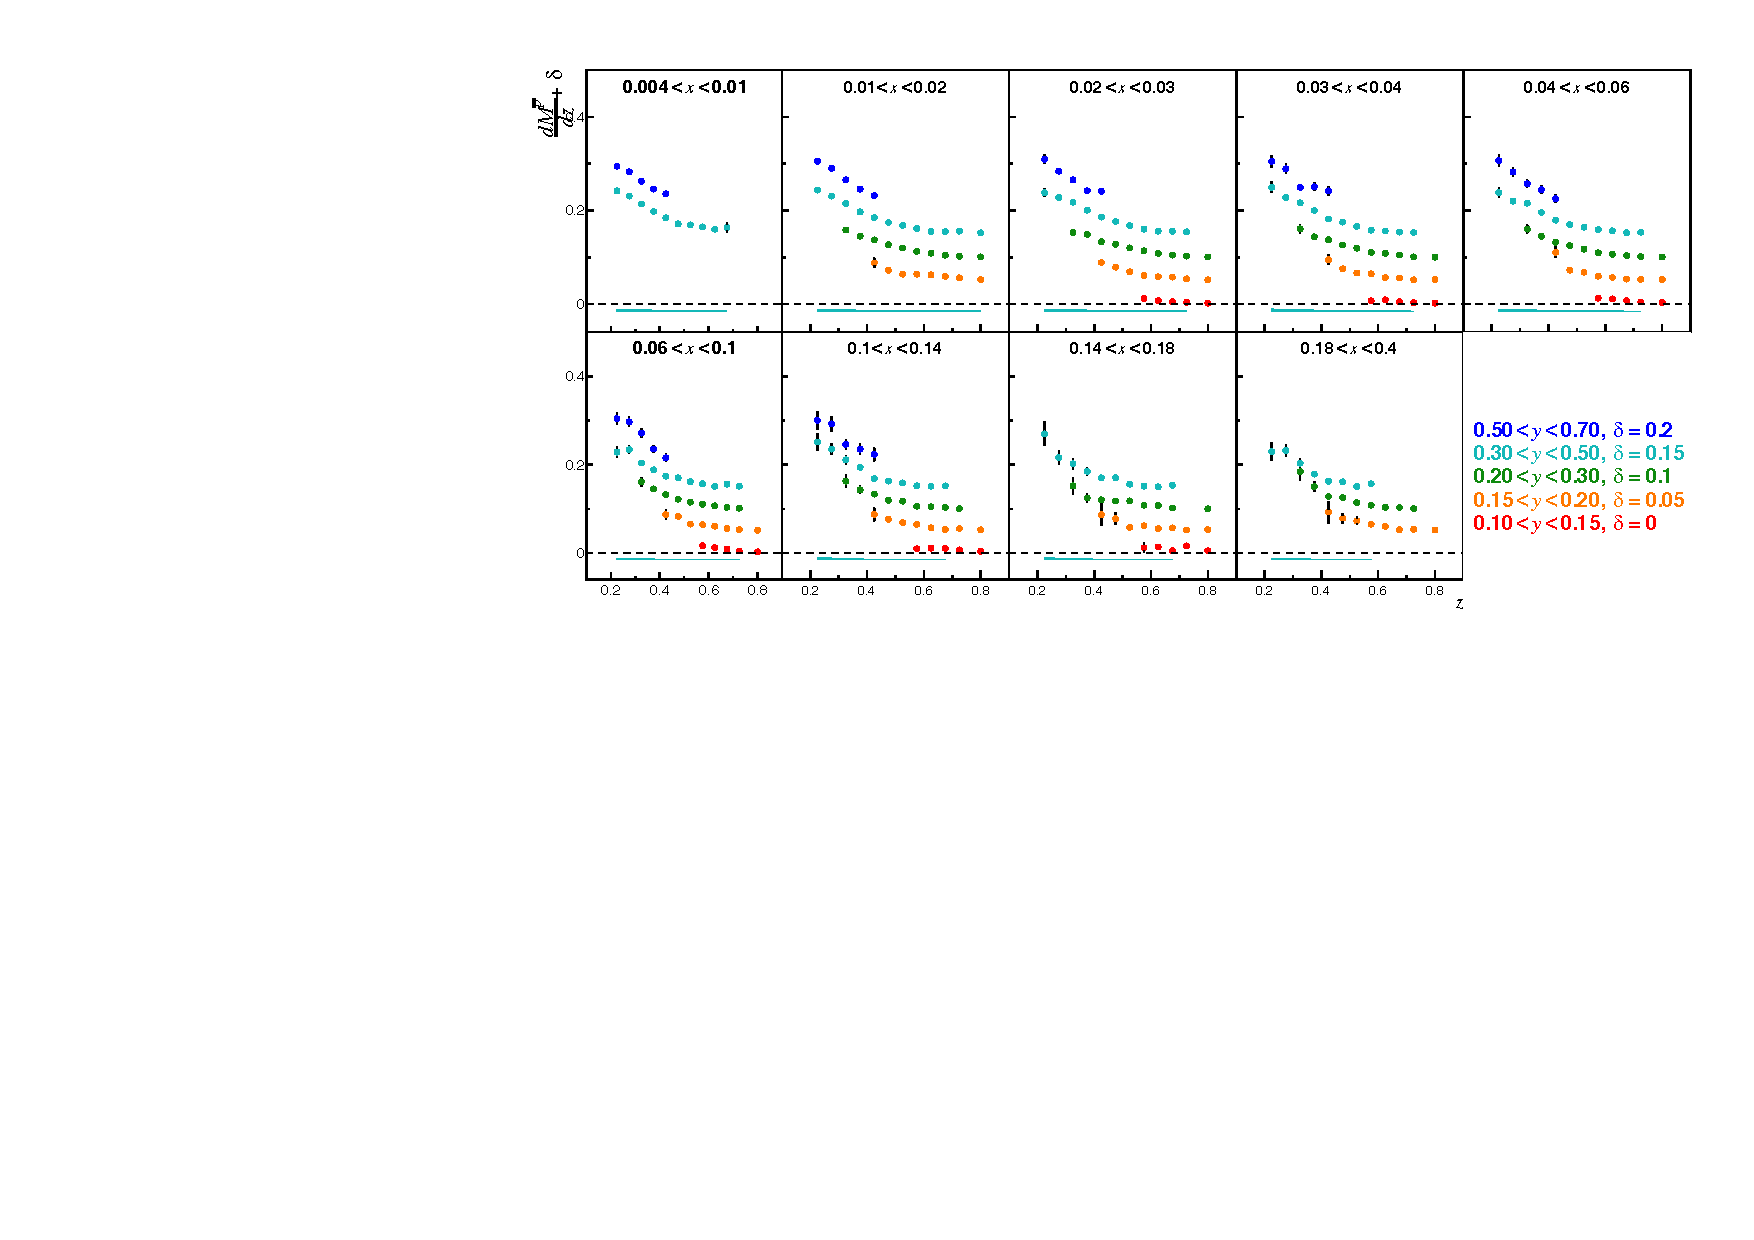
\includegraphics[scale=0.85]{./gfx/pm.pdf}
	\caption{Antiproton multiplicities (with all corrections) as a function of $z$ in bins of $x$ staggered vertically with $y$.}
	\label{pic:mpm}
\end{figure}

The y-averaged multiplicities are displayed as a function of $z$ and in bins of $x$. With Fig. \ref{pic:mpyavg} an asymmetry between $K^+$ and $K^-$ is observed, increasing with $x$. Having more $K^+$ than $K^-$ is due to the fact there is a dominant $u$ quark distribution in the target.

\begin{figure}[!h]
	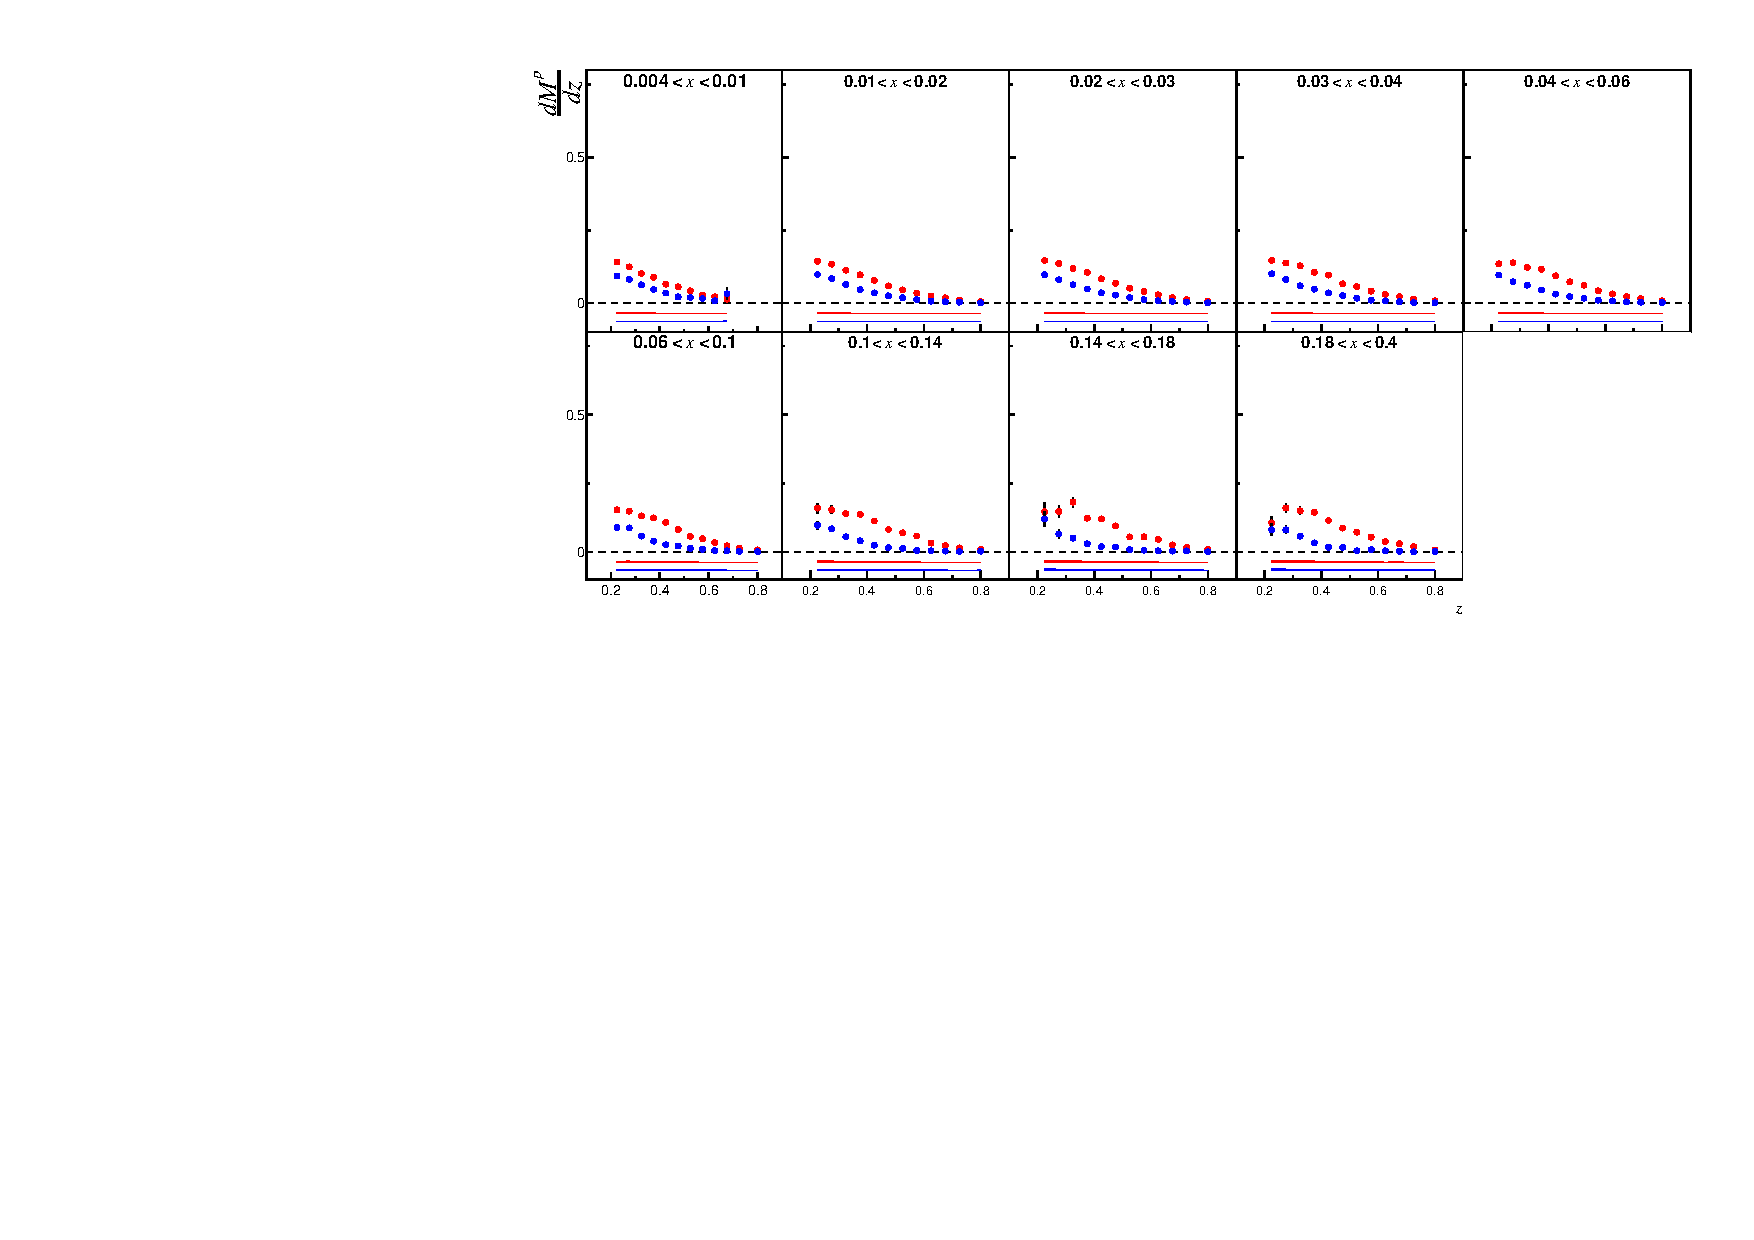
\includegraphics[scale=0.85]{./gfx/pyavg.pdf}
	\caption{Proton (red) and antiproton (blue) multiplicities (with all corrections) averaged over $y$ as a function of $z$ in bins of $x$.}
	\label{pic:mpyavg}
\end{figure}

\section{Ratio of charged hadron multiplicities}

From the $y$-averaged multiplicities, we can still integrate on $z$ to get rid of the $z$ dependence and be able to compare our results with other experiment and also have a scent of the physic underlying. One interesting quantity to look at is the ratio of charged hadron multiplicities as with this quantity most of the systematics cancel by and large. The ratio is calculated as following :

\begin{equation}
  \frac{\mathscr{M}^{h^+}}{\mathscr{M}^{h^-}} = \frac{\int_{0.2}^{0.85} \langle M^{h^+} \rangle_y dz}{\int_{0.2}^{0.85} \langle M^{h^-} \rangle_y dz}
\end{equation}

Only the 8 $x$ bins that have a sufficient $z$ coverage subsist.

\subsection{Ratio of unidentified charged hadron multiplicities}

\begin{figure}[!h]
	\includegraphics[scale=0.5]{./gfx/hr.png}
	\caption{Ratio of $\frac{\mathscr{M}^{h^+}}{\mathscr{M}^{h^-}}$ for COMPASS on proton target (blue closed points) and isoscalar target (orange closed points).}
	\label{pic:hratio}
\end{figure}

The hadron ratio on proton target should lie above COMPASS results on isoscalar target, the reason being the different quark mixture in the two targets (more $u$ in proton target thus higher $\pi+$/$\pi-$ ratio in proton than in isoscalar). The difference is expected to be $\sim$10-20\%.

\subsection{Ratio of charged pion multiplicities}

\begin{figure}[!h]
	\includegraphics[scale=0.5]{./gfx/pir.png}
	\caption{Ratio of $\frac{\mathscr{M}^{\pi^+}}{\mathscr{M}^{\pi^-}}$ for COMPASS on proton target (blue closed points) and isoscalar target (orange closed points) and for HERMES on proton target (violet open points) and deuteron target (green open points).}
	\label{pic:piratio}
\end{figure}

For the very same reason as for hadron, the pion ratio on proton target is expected to be bigger than COMPASS results on isoscalar target by $\sim$10-20\%.

\subsection{Ratio of charged kaon multiplicities}

\begin{figure}[!h]
	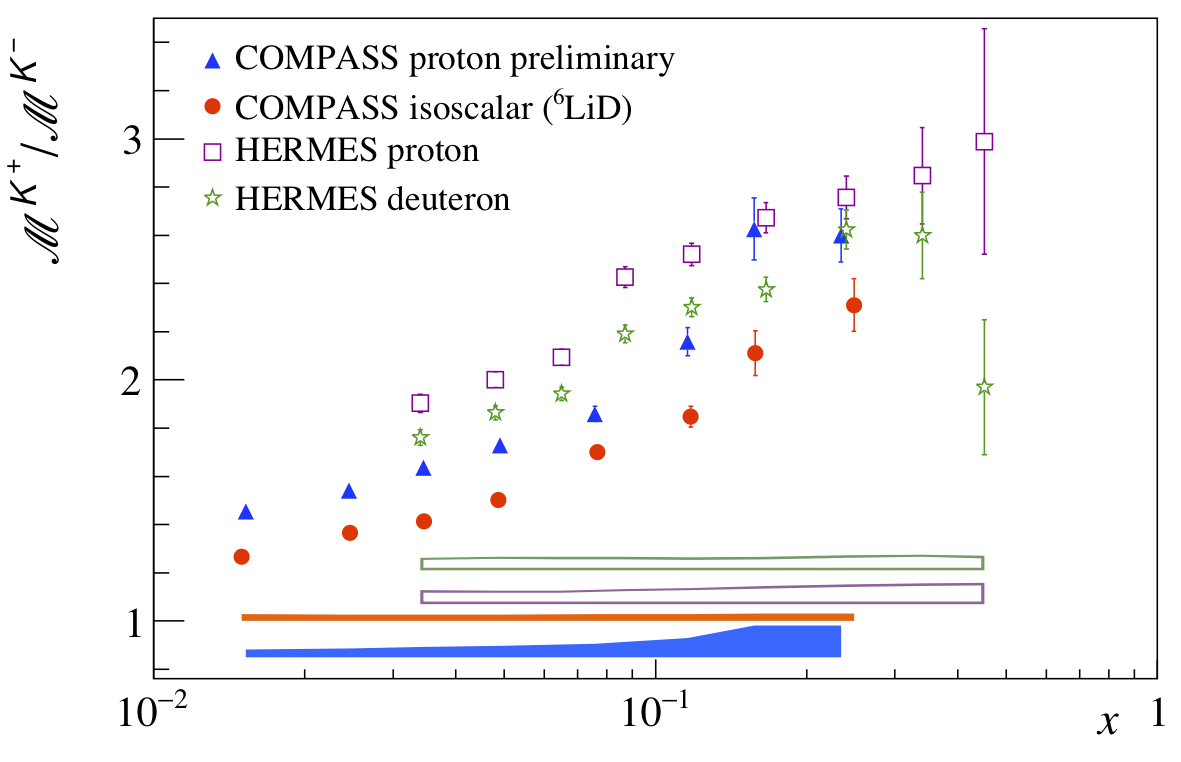
\includegraphics[scale=0.5]{./gfx/Kr.png}
	\caption{Ratio of $\frac{\mathscr{M}^{K^+}}{\mathscr{M}^{K^-}}$ for COMPASS on proton target (blue closed points) and isoscalar target (orange closed points) and for HERMES on proton target (violet open points) and deuteron target (green open points).}
	\label{pic:kratio}
\end{figure}

For the very same reason as for hadron and pion, the kaon ratio on proton target is expected to be bigger than COMPASS results on isoscalar target by $\sim$10\%.

\subsection{Ratio of proton/anitproton multiplicities}

\begin{figure}[!h]
	\includegraphics[scale=0.5]{./gfx/pr.png}
	\caption{Ratio of $\frac{\mathscr{M}^{p}}{\mathscr{M}^{\overline{p}}}$ for COMPASS on proton target (blue closed points).}
	\label{pic:pratio}
\end{figure}

\section{Sum of charged hadron multiplicities}

One other interesting quantity to look at is the sum of charged hadron multiplicities as for some type of hadrons, the results between the multiplicities extracted on a proton target ($lH_2$, this analysis) and an isoscalar target ($^6LiD$, COMPASS published results) should be similar.

All the 2016 results for the sum seem to suffer from a drop a high $x$, particularly visible on hadrons and pions. The kaons seem to be less harmed by this issue. The cause of this drop is still under investigation and might probably be caused by a bad tuning of some hadron variables like $\theta_h$. In the 2006 analysis, the high-$p_T$ tuning of the Monte-Carlo simulation was giving solid description for this variable when in the 2016 analysis, with the same tuning, there is a great discrepancy between data and Monte-Carlo that might play a role in the aforementionned issue.

\subsection{Sum of unidentified charged hadron multiplicities}

\begin{figure}[!h]
	\includegraphics[scale=0.5]{./gfx/hs.png}
	\caption{Sum of $\mathscr{M}^{h^+}+\mathscr{M}^{h^-}$ for COMPASS on proton target (blue closed points) and isoscalar target (orange closed points).}
	\label{pic:hsum}
\end{figure}

The hadron sum for proton target should lie at the same level than COMPASS results on isoscalar target. The discrepancy in amplitude can be explained by the fact that the radiative correction at the time of the publication were not correct and with our nowadays knowledge of radiative corrections, we know that all the points should be moved up by $\sim$6\%, which reconciles proton and isoscalar results within error bars, at least for low $x$. At high $x$ for the results on proton target, the problem comes likely from a bad description of semi-inclusive variable in the Monte-Carlo.

\subsection{Sum of charged pion multiplicities}

\begin{figure}[!h]
  \includegraphics[scale=0.5]{./gfx/pis.png}
  \caption{Sum of $\mathscr{M}^{\pi^+}+\mathscr{M}^{\pi^-}$ for COMPASS on proton target (blue closed points) and isoscalar target (orange closed points) and for HERMES on proton target (violet open points) and deuteron target (green open points).}
  \label{pic:pisum}
\end{figure}

The pion sum for proton target should lie at the same level than COMPASS results on isoscalar target. The same reasoning can be done as in the hadron case, which reconcile at low $x$ at least the COMPASS results on proton target and on isoscalar target.

\subsection{Sum of charged kaon multiplicities}

\begin{figure}[!h]
  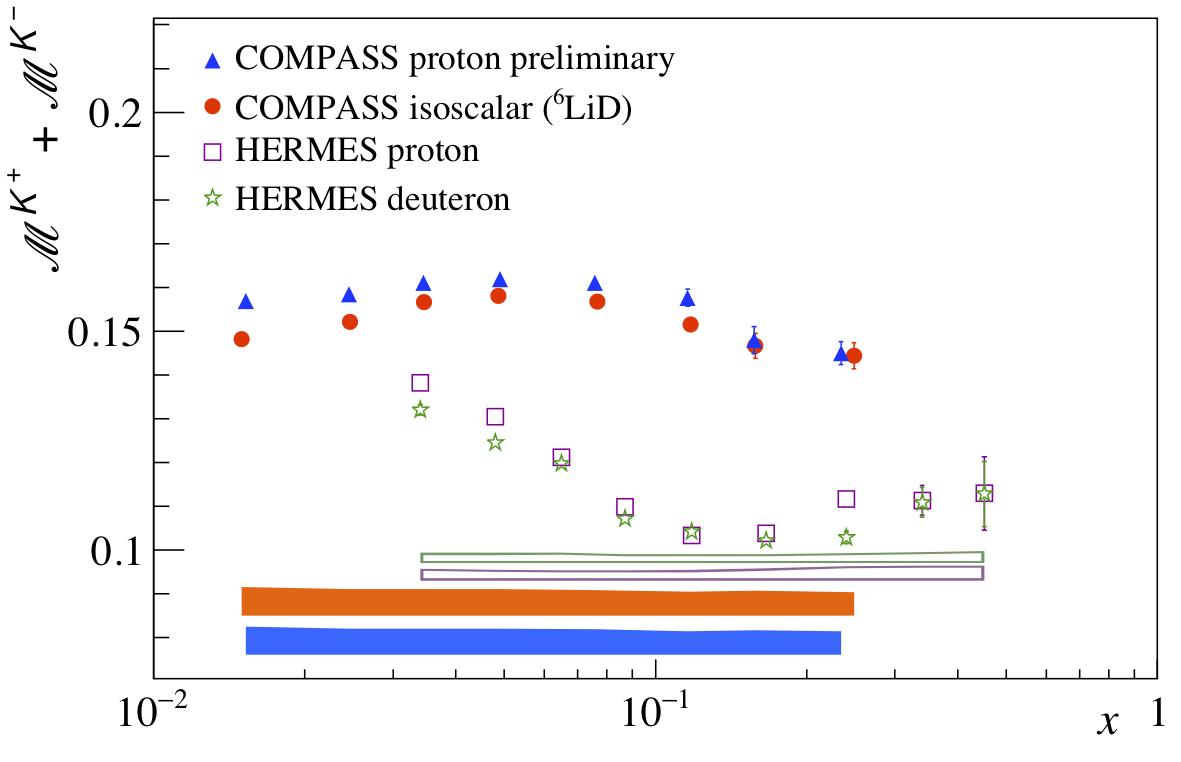
\includegraphics[scale=0.5]{./gfx/Ks.png}
  \caption{Sum of $\mathscr{M}^{K^+}+\mathscr{M}^{K^-}$ for COMPASS on proton target (blue closed points) and isoscalar target (orange closed points) and for HERMES on proton target (violet open points) and deuteron target (green open points).}
  \label{pic:ksum}
\end{figure}

The kaon sum for proton target should be slightly ($\sim$5-10\%) above COMPASS results on isoscalar target. For the isoscalar results for kaons, contrary to hadrons and pions, an additional $5\%$ was added to the published results to take into account the bad knowledge of the radiative correction at the time. The discrepancy with HERMES results, already seen in the isoscalar case, remains.

\subsection{Sum of proton/antiproton multiplicities}

\begin{figure}[!h]
	\includegraphics[scale=0.5]{./gfx/ps.png}
	\caption{Sum of $\mathscr{M}^{p}+\mathscr{M}^{\overline{p}}$ for COMPASS on proton target (blue closed points).}
	\label{pic:psum}
\end{figure}

\section{Summary}
